\documentclass[12pt,a4paper]{article}

%% --- Encoding and fonts ---
\usepackage[utf8]{inputenc}
\usepackage[T1]{fontenc}
%\usepackage{lmodern}  % disabled for review copy: newpx loaded by paper_style_preamble

%% --- Language ---
\usepackage[english]{babel}

%% --- Mathematics ---
\usepackage{amsmath, amssymb, amsthm}
\usepackage{mathtools}

%% --- Layout ---
\usepackage[margin=1in]{geometry}
\usepackage{setspace}
\onehalfspacing

%% --- Figures and tables ---
\usepackage{graphicx}
\usepackage{booktabs}
\usepackage{caption}
\usepackage{subcaption}
\usepackage{float}

%% --- Appendix ---
\usepackage[title,titletoc]{appendix}

%% --- Cross-references and links ---
\usepackage{hyperref}

%% --- Bibliography ---
\usepackage{natbib}
\bibliographystyle{apalike}

%% --- Draft tools ---
\usepackage{xcolor}
\newcommand{\todo}[1]{\textcolor{red}{\textbf{[TODO: #1]}}}
\newcommand{\note}[1]{\textcolor{blue}{\textit{[Note: #1]}}}

%% --- Paper style (splice review copy): Carrasco-2026 look ---
% ======================================================================
% paper_style_preamble.tex — drop-in style fragment (Carrasco 2026 look)
% ======================================================================
% Anchor: carrasco2026.pdf (repo root). Colors below were extracted from
% that PDF's content streams, not eyeballed:
%   citations / URLs   RGB(162, 99, 49)  = #A26331 (sienna)
%   internal links     RGB( 48, 73, 89)  = #304959 (dark slate)
%   figure series      #3C5B6F (slate navy) / #BA8F6B (muted copper),
%                      darker accents #1A476F / #B36633; gridlines 50% grey
% The matplotlib mirror of the figure palette is paper_plot_style.py.
%
% HOW TO USE WITH Draft_august.tex
%   1. DELETE (or comment out) \usepackage{lmodern} in the main preamble.
%      Palatino (newpx) and Latin Modern fight over the text font; the
%      last one loaded wins and the metrics disagree. This fragment loads
%      newpxtext/newpxmath (fallback: mathpazo).
%   2. \input{style/paper_style_preamble} AFTER the
%      existing package block. It is compatible with the rest of
%      Draft_august's preamble (amsmath/amssymb/mathtools, geometry,
%      setspace, graphicx, booktabs, caption, subcaption, float,
%      appendix, natbib, xcolor): everything here either loads a package
%      not already present or only calls \hypersetup / \captionsetup.
%   3. DELETE the existing \hypersetup{colorlinks=true, linkcolor=blue,
%      citecolor=blue, urlcolor=blue} line — this fragment replaces it.
%      (If hyperref is not yet loaded, this fragment loads it.)
% ======================================================================

% ---- Typography: Palatino text + matching math (Carrasco uses the
%      Palatino family; newpx is the maintained implementation) ---------
\IfFileExists{newpxtext.sty}{%
  \usepackage{newpxtext}%
  \usepackage{newpxmath}%
}{%
  \usepackage{mathpazo}% fallback: Palatino text + math
}
\linespread{1.18} % Palatino needs more leading; approximates the anchor's
                  % openness without double-spacing (setspace, if loaded,
                  % may override this — call \onehalfspacing after if desired)
\setlength{\emergencystretch}{1.5em} % Palatino sets wider than CM/LM;
                  % this absorbs the overfull lines the font swap creates

% ---- Colors (extracted from carrasco2026.pdf) ------------------------
\usepackage{xcolor} % no-op if already loaded
\definecolor{citesienna}{RGB}{162, 99, 49}   % citations, URLs
\definecolor{linkslate}{RGB}{48, 73, 89}     % internal refs (sections, eqs, tables)
\definecolor{sernavy}{RGB}{26, 71, 111}      % figure series 1 (dark navy)
\definecolor{sercopper}{RGB}{179, 102, 51}   % figure series 2 (burnt sienna)
\definecolor{sernavyline}{RGB}{60, 91, 111}  % muted line variant of series 1
\definecolor{sercopperline}{RGB}{186, 143, 107} % muted line variant of series 2

% ---- Hyperref: colored author-year citations, slate internal links ---
\makeatletter
\@ifpackageloaded{hyperref}{}{\usepackage{hyperref}}
\makeatother
\hypersetup{
  colorlinks = true,
  citecolor  = citesienna,
  urlcolor   = citesienna,
  linkcolor  = linkslate,
  filecolor  = linkslate,
}

% ---- Captions: "Table 1: Baseline calibration" above tables/figures,
%      slightly smaller than body, plain weight (anchor style) ---------
\makeatletter
\@ifpackageloaded{caption}{}{\usepackage{caption}}
\makeatother
\captionsetup{labelsep=colon, font=small, labelfont=bf, skip=6pt}
% Anchor convention: captions sit ABOVE tables and ABOVE figures.
% (Position is set where the float is written, not here.)

% ---- Tables: booktabs + the Carrasco Table-1 idiom -------------------
\makeatletter
\@ifpackageloaded{booktabs}{}{\usepackage{booktabs}}
\makeatother

% Small-caps column heads: \thead{Description} -> DESCRIPTION in
% spaced small caps, the anchor's header style.
\newcommand{\thead}[1]{\multicolumn{1}{c}{\footnotesize\textsc{#1}}}
\newcommand{\theadl}[1]{\multicolumn{1}{l}{\footnotesize\textsc{#1}}}
\newcommand{\theadr}[1]{\multicolumn{1}{r}{\footnotesize\textsc{#1}}}

% Bold full-width group-separator row: \tgroup{4}{Demographics and Healthcare}
% (first argument = number of columns in the tabular).
\newcommand{\tgroup}[2]{\multicolumn{#1}{l}{\textbf{#2}}\\}

% Under-table notes minipage: \tabnote{0.92}{...} — bold run-in "Notes."
% then footnotesize flowing text, width as a fraction of \textwidth.
\newcommand{\tabnote}[2]{%
  \vspace{0.5em}\par
  \begin{minipage}{#1\textwidth}
  \footnotesize\emph{Notes.} #2
  \end{minipage}}

% Under-figure note, anchor style ("Note." then series names in their
% colors): \fignote{0.9}{Expenditure ... \serone{Top 10 percent} and
% \sertwo{Bottom 90 percent}.}
\newcommand{\fignote}[2]{%
  \vspace{0.4em}\par
  \begin{minipage}{#1\textwidth}
  \footnotesize\textbf{Note.} #2
  \end{minipage}}
\newcommand{\serone}[1]{\textcolor{sernavy}{#1}}
\newcommand{\sertwo}[1]{\textcolor{sercopper}{#1}}

% ----------------------------------------------------------------------
% TEMPLATE — the Carrasco Table-1 skeleton (baseline-calibration table).
% Copy, uncomment, fill. Structure: caption ABOVE; four columns
% (symbol | description | value | target/source); small-caps heads;
% bold group rows separating parameter families; sources as \citep{}
% (they render sienna); notes minipage below.
% ----------------------------------------------------------------------
% \begin{table}[H]
% \centering
% \caption{Baseline calibration}
% \label{tab:baseline_calibration}
% \begin{tabular}{@{}llcl@{}}
% \toprule
%  & \theadl{Description} & \thead{Value} & \theadr{Target/Source} \\
% \midrule
% \tgroup{4}{Demographics and Healthcare}
% $n$              & Fertility rate            & $0.03$      & Population growth $=1\%$ \\
% $\bar\psi$       & Survival rate parameters  & See text    & WPP, HRS, MEPS \\
% \tgroup{4}{Preferences}
% $\beta$          & Subjective discount rate  & Internally calibrated & Interest rate $4\%$ (p.a.) \\
% $\sigma$         & Risk aversion             & $2.0$       & \citep{SomeSource2019} \\
% \bottomrule
% \end{tabular}
% \tabnote{0.92}{Rates are annual. Internally calibrated parameters are
% estimated in Section~X; see Table~Y.}
% \end{table}
% ----------------------------------------------------------------------

\newcommand{\TODO}[1]{\textbf{[TBD#1]}}
% --- Custom Math Commands ---
\newcommand{\E}{\mathbb{E}}
% Type-specific shortcuts
\newcommand{\tL}{\theta_L}
\newcommand{\tH}{\theta_H}

%% --- Theorem environments ---
\newtheorem{definition}{Definition}

%% ====================================================================
\begin{document}

%% --- Title block ---
\title{\textbf{Spending Smarter under Demographic Pressure:}\\[6pt]
Fiscal Efficiency, Health, and Gender Dynamics\\
in Latin America\thanks{The work was financed with the support of the Latin America and the Caribbean Research Network of the Inter-American Development Bank. The opinions expressed in this publication are those of the authors and do not necessarily reflect the views of the Inter-American Development Bank, its Board of Directors, or the countries they represent.}}

\author{
Diego Ascarza-Mendoza\textsuperscript{1} \quad Hermilo Cort\'es\textsuperscript{2}\\[3pt]
Judith M\'endez\textsuperscript{2} \quad H\'ector J.\ Villarreal\textsuperscript{2}
\\[6pt]
\textsuperscript{1}Carleton College\\
\textsuperscript{2}Iniciativa para la Transici\'on Econ\'omica y Demogr\'afica (ITED),\\
Escuela de Gobierno y Transformaci\'on P\'ublica,\\
Tecnol\'ogico de Monterrey
}
\date{%
Prepared for the Inter-American Development Bank,\\
Fiscal Division\\[12pt]
\textit{Preliminary draft -- August 2026}\\
\textit{Please do not cite or circulate without permission}
}

\maketitle

%% --- Abstract ---


\begin{abstract}
This paper examines the macroeconomic and welfare consequences of demographic aging under alternative pension adjustments in Mexico. We use a calibrated stochastic overlapping-generations general-equilibrium model with endogenous health investment and heterogeneity by sex and education. Comparing stationary equilibria under the projected 2050 old-age dependency ratio, we find that maintaining the pension replacement rate and retirement age raises the contribution rate from $5.66\%$ to $12.26\%$. Capital deepening raises wages but leaves aggregate newborn welfare nearly unchanged relative to 2020, while welfare comparisons for older residents become increasingly negative. Relative to this contribution-rate adjustment, reducing the replacement rate from $0.40$ to $0.185$ increases newborn welfare by $8.29\%$. Lower pension benefits encourage private saving and capital deepening, while higher wages and lower contributions offset the reduction in benefits for newborns. Raising the retirement age from 65 to 70 increases newborn welfare by $3.11\%$, as a broader contribution base and fewer pension recipients reduce required contributions. Both reforms benefit newborns across sex-education groups, but their age-specific welfare consequences differ, particularly for pension-dependent older residents and low-education women approaching retirement. 
\end{abstract}


\noindent\textbf{Keywords:} demographic transition; fiscal sustainability; social security; pension reform; health capital; overlapping generations; Latin America

\noindent\textbf{JEL codes:} E62, H55, I13, J11, J26

%% ====================================================================
%% SECTION 1 — INTRODUCTION
%% ====================================================================


\section{Introduction}
\label{sec:intro}

Mexico's old-age dependency ratio is projected to more than double between 2020 and 2050, from $0.141$ to $0.307$ \citep{CONAPO2023}. In a balanced pay-as-you-go pension system, an increase in the ratio of retirees to working-age individuals requires higher payroll contributions if the replacement rate and retirement age remain unchanged. Alternatively, the adjustment can be accommodated through lower pension benefits or later retirement. These alternatives have different implications for household saving, labor supply, and the distribution of resources across generations, while also affecting equilibrium wages and interest rates. In this paper, we quantify the macroeconomic and welfare consequences of demographic aging under these alternative pension adjustments in Mexico.

To examine these interactions, we develop a quantitative stochastic overlapping-generations general-equilibrium model calibrated to the Mexican economy. Households differ by sex, education, and idiosyncratic productivity, and make life-cycle decisions about consumption, saving, labor supply, and medical spending. Medical spending affects health, which in turn influences survival probabilities, labor productivity, and utility. Household saving and labor supply decisions determine aggregate capital and effective labor, and hence equilibrium wages and interest rates. The model incorporates a pay-as-you-go pension system, allowing us to examine how alternative pension adjustments affect household decisions and welfare through changes in pension benefits, payroll contributions, and equilibrium factor prices.

We discipline the model using Mexican data on life-cycle earnings, medical spending, and survival. The National Survey of Household Income and Expenditure (ENIGH) provides earnings profiles by age, sex, and education, as well as information on how medical spending varies with age and income. The Mexican Health and Aging Study (ENASEM) provides evidence on health deterioration and mortality differences across demographic groups. We combine these data with demographic, production, and fiscal parameters obtained from official statistics and existing research. We calibrate the model using patterns of medical spending over the life cycle, earnings differences by sex and education, and survival probabilities across demographic groups.


Our first experiment examines demographic aging under the contribution-rate adjustment, which maintains the replacement rate and retirement age at their baseline levels. The pension contribution rate increases from $5.66\%$ to $12.26\%$. At the same time, population aging leads to capital deepening, raising wages by $12.4\%$ and reducing the annual interest rate from $8.58\%$ to $6.82\%$. These changes have offsetting effects on household welfare. Despite the substantial increase in pension contributions, aggregate newborn welfare increases by only $0.14\%$ of lifetime consumption relative to the 2020 baseline. The age-specific welfare comparisons reveal a different pattern. Relative to the 2020 equilibrium, residents of the aged economy experience increasingly large welfare losses at older ages, reaching $12$--$21\%$ of remaining lifetime consumption at ages 65--69.

Using the calibrated model, we first examine the effects of demographic aging when the pension system adjusts through higher payroll contributions, holding the replacement rate and retirement age unchanged. The contribution rate increases from $5.66\%$ to $12.26\%$. At the same time, demographic aging leads to capital deepening, raising wages by $12.4\%$ and reducing the annual interest rate from $8.58\%$ to $6.82\%$. These changes have offsetting effects on household welfare, leaving aggregate newborn welfare nearly unchanged, with a consumption-equivalent gain of $0.14\%$ relative to the 2020 baseline. However, the age-specific welfare comparisons reveal substantial differences. Relative to the 2020 equilibrium, residents of the aged stationary economy experience increasingly large welfare losses at older ages, reaching $12$--$21\%$ of remaining lifetime consumption at ages 65--69.

We next examine two alternative pension reforms under the same demographic conditions. Reducing the pension replacement rate from $0.40$ to approximately $0.185$ restores the contribution rate to its 2020 level and increases aggregate newborn welfare by $8.29\%$ relative to contribution-rate adjustment. Raising the retirement age from 65 to 70 reduces the contribution rate to $8.78\%$ and generates a newborn welfare gain of $3.11\%$ relative to contribution-rate adjustment. The benefit reduction encourages private saving and generates additional capital deepening, raising wages and lowering interest rates. In contrast, raising the retirement age increases capital and effective labor in similar proportions, leaving factor prices nearly unchanged.

The welfare consequences of these adjustments also differ substantially by sex and education, particularly at older ages. Under contribution-rate adjustment, welfare losses among older residents are greatest for high-education households, which hold more assets and are more exposed to the decline in interest rates. In contrast, reducing pension benefits generates larger losses among households that rely more heavily on pension income. For example, at ages 65--69, low-education women experience welfare losses equivalent to approximately $21\%$ of remaining lifetime consumption, compared with $3.7\%$ for high-education men. Raising the retirement age also disproportionately affects low-education women, whose welfare at ages 65--69 declines by $9.5\%$, while high-education individuals experience welfare gains across all ages. These findings highlight the importance of differences in life-cycle earnings, asset accumulation, and survival across sex and education groups for evaluating the distributional consequences of pension reform.

Our paper contributes to the quantitative literature on demographic aging and pension reform by examining their welfare consequences in Mexico, with particular attention to differences across age, sex, and education. Previous studies have analyzed the general-equilibrium effects of demographic aging and alternative pension policies \citep{KruegerLudwig2007,Kitao2014}. We extend this analysis to a model calibrated to the Mexican economy, in which the pension contribution rate adjusts endogenously to demographic change and households differ in their life-cycle earnings and survival probabilities. These differences allow us to examine how changes in pension benefits, contributions, and returns on savings affect the welfare of different demographic groups. Our framework also incorporates endogenous medical spending, through which health influences labor productivity and longevity. Related overlapping-generations models have studied endogenous health in general equilibrium \citep{JungTranChambers2017}, while \citet{CortesEtAl2024} examines health heterogeneity in Mexico in partial equilibrium. We bring these elements together to evaluate the aggregate and distributional consequences of alternative pension adjustments in a common quantitative framework.

The remainder of the paper is organized as follows. Section~\ref{sec:lit} reviews the related literature. Section~\ref{sec:model} presents the model, and Section~\ref{sec:calibration} describes its calibration and evaluates its quantitative performance. Section~\ref{sec:experiments} presents the counterfactual experiments, and Section~\ref{sec:conclusion} concludes.


%% ====================================================================
%% SECTION 2 — LITERATURE REVIEW
%% ====================================================================
\section{Literature Review}
\label{sec:lit}

This paper draws on four literatures. The first is the quantitative
overlapping-generations literature on demographic aging and pension reform,
which supplies the questions the paper answers and the benchmarks against which
its answers are read. The second is the literature that models health as a
capital stock built by forward-looking investment, which supplies the apparatus.
The third fixes the institutional environment in which health and pensions are
financed in Latin America and bounds what the model can be asked. The fourth
locates the heterogeneity by sex and education through which every incidence
result in the paper is priced. They are not treated at equal depth: the review
is weighted toward the first, second, and fourth, where the paper's
contributions lie.

%% --------------------------------------------------------------------
\subsection{Aging, Pension Reform, and Incidence in Quantitative Over\-lapping-Generations Models}
\label{subsec:lit_pension}

Since \citet{AuerbachKotlikoff1987}, the workhorse for analyzing the
intergenerational fiscal consequences of demographic change has been the
multi-period overlapping-generations model with a government sector, and three
threads of that literature organize this paper's principal results.

The first is the transmission of aging to welfare through factor prices.
\citet{KruegerLudwig2007} establish the central result: population aging raises
the capital--labor ratio, so wages rise and returns fall, and the welfare
consequences split by what a household holds---agents whose lifetime resources
are mostly labor income gain, while cohorts already holding assets lose as their
wealth is repriced at the lower return. This paper's first finding is that mechanism, obtained for Mexico. Where \citet{KruegerLudwig2007} show that the adjustment of the contribution rate can offset the direct effect of aging, we price that offset at an estimated emerging-economy baseline and resolve its incidence by age, sex, and education: because our pay-as-you-go contribution rate adjusts to balance the system, aging arrives at the household simultaneously as a factor-price change and as a doubled tax wedge, and the newborn's near-indifference is the net of the two. \citet{CarvalhoFerreroNechio2016} separate the channels through
which aging moves the equilibrium return---longevity and the dependency ratio---a decomposition directly relevant here, since our
demographic experiment moves fertility only and holds survival at its estimated
schedules. \citet{AuclertEtAl2021} quantify these forces at the frontier and
across countries, and their finding that the sign and size of the aging effect
depend heavily on country characteristics is the reason an emerging-economy
calibration is not a mechanical application of the high-income results.

The second thread is the reform menu itself. \citet{Kitao2014} enumerates the
options for restoring pay-as-you-go sustainability under aging---raising the
payroll tax, cutting the replacement rate, raising the retirement age, and
means-testing benefits---and prices them in a general-equilibrium life-cycle
model. Our menu is Kitao's minus means-testing, which the flat benefit of
Section~\ref{sec:model} cannot represent, and the omission is a property of the
benefit rule rather than a judgment about the instrument. That the choice among
pension architectures is fundamentally distributional, and can be posed as a
comparison across stationary economies, is established by
\citet{HuggettVentura1999}; their exercise is the precedent for our own
restriction to steady states. Two papers supply the counterweight that
disciplines how our welfare rankings may be read.
\citet{ConesaKrueger1999} and \citet{NishiyamaSmetters2007} establish that an unfunded pillar provides insurance against uninsurable idiosyncratic wage risk: \citet{NishiyamaSmetters2007} show that the efficiency gains from shrinking it reverse once that insurance is priced, and \citet{ConesaKrueger1999} that it is what sustains political support for the status quo.

The third thread is differential mortality. \citet{SanchezRomeroEtAl2020} show
that longevity gaps by socioeconomic status transfer resources toward the
long-lived and undermine the actuarial fairness of pension systems; their paper is the
closest existing work to this paper's finding that the education gradient in
survival decides which type loses under inaction. \citet{Bagchi2019} supplies
the caution, finding that optimal progressivity is surprisingly insensitive to
wealth-dependent mortality---a result worth holding against ours, which reports
an incidence pattern rather than an optimal policy.

Two further anchors bound the exercise. Every welfare ranking below rests on the
condition of \citet{Aaron1966}: where the market return exceeds the growth rate
of the contribution base, mandatory participation in an unfunded pillar
transfers resources away from the participant. Whether that condition holds is not settled by assumption, and \citet{AbelEtAl1989} show that the comparison is delicate once uncertainty is admitted; in the deterministic aggregate environment of this model the gap is direct, and the annual return ranges from $5.89$ to $8.58$ percent against base growth of at most $3.51$ percent, so the condition holds with room to spare in every economy on the menu. And the factor-price channel that carries
our first finding is a closed-economy object. \citet{AttanasioKitaoViolante2007}
show that capital mobility between asynchronously aging regions substantially
mitigates the factor-price consequences of aging, and that the South's exposure
differs from the North's; we treat the closed-economy assumption as this paper's
most fragile and flag it where the results depend on it. For the regional fiscal
scale of the problem, \citet{PessinoTerMinassian2021} project pension and health
spending pressure across Latin America over a fifty-year horizon.

This paper's contribution to this literature is to price all three feasible margins side by side, in one estimated general equilibrium for an emerging economy,
with incidence resolved by age, sex, and education through schedules that enter
from the data rather than from assumption. One bound on that contribution should be stated here rather than discovered later. Our welfare comparisons price the return gap of the Aaron condition between stationary economies, but they do not price the journey between them: the newborn gain we report from cutting benefits accrues to a newborn of the reformed steady state who never contributed at the old rate, and on the evidence of \citet{NishiyamaSmetters2007}, who compensate transitional losses explicitly, it should be read as an upper bound on what that reform is worth.

%% --------------------------------------------------------------------
\subsection{Health, Longevity, and the Life Cycle}
\label{subsec:lit_longevity}

The apparatus this paper builds descends from \citet{Grossman1972}, and the
inheritance should be stated as an assumption rather than absorbed as a
convention: health is a depreciable capital stock, medical spending is
forward-looking investment in that stock, and the stock so built governs
survival and---in the richer versions---labor productivity. Four functions have
been asked of that block, and the literature is best read by which one a given
paper assigns it.

The first is to generate aging and mortality endogenously.
\citet{DalgaardStrulik2014} derive the pattern of aging and death from the
interaction of health investment with biological depreciation, yielding a
structural reading of the Preston curve; \citet{KuhnFeichtinger2015} analyze
health and retirement choices jointly when health capital depreciates with age
and can be partially restored; and \citet{Fioroni2010} shows that the
interaction of precautionary saving with health investment produces
consumption--saving profiles unlike those of models with exogenous health. The
second function is to price life itself. \citet{HallJones2007} show that when
health enters preferences so that the marginal value of additional life rises
with consumption, the aggregate income elasticity of health spending exceeds one and
health's expenditure share grows with development; \citet{MurphyTopel2006}
develop the same valuation structure and its empirical magnitudes. This paper's
multiplicative health amenity, and the income gradient in willingness to pay
for health it generates, is that mechanism embedded in a general-equilibrium
life cycle.

The third function is to close a macroeconomic loop. \citet{JungTran2016} and \citet{JungTranChambers2017} build stochastic general-equilibrium overlapping-generations economies with endogenous health capital and health insurance; \citet{JungTranChambers2017} use that apparatus for aging experiments---the closest existing statement of
the apparatus combination this paper claims, executed for the United States.
\citet{Zhao2014} closes the loop in the other direction, showing that social
security itself alters health investment and longevity, while
\citet{FrankovicWrzaczek2020} trace medical progress through capital
accumulation and factor prices, \citet{YewZhang2018} introduce longevity
externalities, \citet{Lim2020} shows that public health insurance reshapes
aggregate saving in Korea, and \citet{Carrasco2026} operates the same block as a
macroeconomic transmission channel in which investment in health lengthens
lives, strengthens life-cycle saving, and moves the equilibrium interest rate.
The fourth function is to carry expenditure risk. \citet{DeNardi2010} show that
uncertain medical expenses are a primary driver of late-life saving among older
American households; \citet{HosseiniKopeckyZhao} estimate the health-deficit
process on United States panel data with health observed from early adulthood;
and \citet{GertlerGruber2002} establish for a developing economy the fact that
motivates the health-risk side of the design---major illness is a large shock that households
insure poorly---although the shocks in our model hit the health stock rather than the household's budget.

The evidentiary base on which the block has been estimated is narrower than its
use. These models are calibrated or estimated overwhelmingly on high-income
data, in economies where coverage is broad and out-of-pocket payments are a
modest share of health spending, so the data do not force a distinction between
spending that builds the stock and spending that repairs it after a shock.
Where that distinction has been confronted, it has been confronted in partial
equilibrium and on United States data: \citet{Ozkan2025} builds a life-cycle
health-capital model that separates preventive from curative spending and
documents how their income gradients differ across the life cycle, and
\citet{GalamaVanKippersluis2013} argue that the standard criticisms of the
Grossman framework rest on a degenerate special case that reformulations
resolve. What has not been attempted is that confrontation inside a general
equilibrium, or on data from an economy in which out-of-pocket payment is an
unusually large share of health spending.

The paper's position here rests on three qualifiers, and the
closest papers are cited so that a reader can check each. \citet{JungTran2016} and
\citet{JungTranChambers2017} deliver the general equilibrium and the endogenous
health stock, but for a high-income economy with broad insurance;
\citet{Zhao2014} delivers the health--fiscal loop, likewise for the United
States; \citet{HosseiniKopeckyZhao} deliver estimation on micro-data, in partial
equilibrium. What this paper adds, for the health block specifically, is the conjunction: a block carrying survival, labor productivity, and the fiscal loop at once, estimated rather than calibrated, in an economy where out-of-pocket payment is an unusually large share of health spending. We claim the combination and not any of its parts---and Section~\ref{subsec:validation} reports how much of the education--survival gradient the investment channel actually generates once the block is estimated.

For the Latin American context, \citet{CortesEtAl2024} develop a
partial-equilibrium overlapping-generations model for Mexico in which agents
differ by skill and face stochastic health transitions, health-dependent
productivity, and age-varying out-of-pocket expenditure. Their
results---consumption gaps of $40$--$70$ percent between good and poor health
groups, and a $20$-year gap in healthy longevity by skill level---establish the
magnitudes at stake in the Mexican setting; the present paper is disciplined
instead against its own ENIGH and ENASEM moments. The extensions are general
equilibrium with endogenous wages, an explicit pension system whose contribution
rate adjusts to balance the system, and heterogeneity by sex as well as skill.

%% --------------------------------------------------------------------
\subsection{Health Financing, Social Insurance, and the Tax Wedge}
\label{subsec:lit_health}

The economics of health insurance in developing economies builds on the insight
that health shocks are both large and poorly insurable through private markets,
generating welfare losses that pooling arrangements can substantially mitigate
\citep{Arrow1963}. In Latin America the design question is not whether to pool
health risk but through which institutional channel. Systems in the Bismarckian
tradition link coverage to formal employment; systems in the Beveridgean
tradition link it to residency or citizenship; and, as \citet{Levy2008}
emphasizes, most countries in the region operate hybrids of the two, often with
fragmentation, duplication, and unequal benefit packages.

\citet{Summers1989} supplies the valuation logic that organizes the modern
literature: mandated contributions are priced into wages and generate no net
distortion when workers value the benefits they purchase, and they function as a
tax on formal labor precisely when workers do not---because benefits are not
credible, or because their arrival is too distant.
\citet{WorldBankInformalizing2025} formalize this logic as the Formalization Tax
Rate, the net fiscal cost of formal employment inclusive of forgone
non-contributory benefits, and show that it is highest for low-income workers,
the group with the weakest attachment to the formal sector. Within this
literature, \citet{BaezaPackard2006} document the asymmetry most relevant to
this paper's design: health coverage delivers immediate, tangible protection
against catastrophic expenditure and is the benefit workers learn most about and
value most highly, while pension benefits arrive far in the future and are
discounted for institutional credibility.

What this subsection establishes for the paper is a boundary rather than a
contribution. The model takes a deliberate position in this landscape: its
pension benefit is flat and indexed to contemporaneous average earnings, so
there is no benefit--contribution link at the individual level---a Beveridgean
benefit inside a Bismarckian financing shell. The simplification buys
tractability in the fiscal block, and it bounds what the paper can say about
formalization incentives, which respond to exactly the individual-level link the
model omits. One feature is worth noting against this literature nonetheless:
the wedge it studies is imposed exogenously in most applications and is determined
by the system's budget here, since the contribution rate balances the pension system
rather than being set.

%% --------------------------------------------------------------------
\subsection{Gender and Education Heterogeneity in Life-Cycle Fiscal Models}
\label{subsec:lit_gender}

Gender-differentiated incidence in social security is an active subject in
estimated life-cycle models. \citet{BorellaDeNardiYang2023} estimate a
life-cycle model of couples and singles with survival risk, medical expenses,
and the marriage-related provisions of United States Social Security, and show
that those provisions carry large and unequal consequences for women's labor
supply and welfare across cohorts. \citet{FehrKindermann2018} provide the
reference framework on the household side, a two-person household whose female
member's labor supply responds to childcare, parental leave, and joint-versus-individual
taxation---but in an environment without health as a state variable,
without endogenous survival, and without a fiscal loop.

The natural extension of that work to this paper's environment has not been
attempted, and the reason is computational rather than conceptual. Embedding a two-earner household of the kind \citet{BorellaDeNardiYang2023} estimate in a
model with continuous health capital, health-modulated survival, and endogenous
factor prices would compound the curse of dimensionality with the fixed-point
problem in prices; to our knowledge no published model carries all four.

The approach here is different, and it is implemented rather than proposed. The
agent space carries four types throughout---two education groups for each
sex---each with its own measured age-efficiency profile and its own baseline
survival schedule, so that the sex- and education-differentiated profiles embed
in reduced form the cumulative effects of labor market histories that a
structural household model would generate endogenously.

Carrying that heterogeneity from measurement through to welfare is one of this
paper's contributions. Quantitative models of pension reform ordinarily resolve
incidence by age and by wealth; resolving it by sex and by education as well
requires survival and efficiency schedules estimated separately for each of the
four groups, and it changes who bears each reform, though not how the reforms rank. Every
experiment below reports welfare and incidence for all four types, and the
patterns that result---low-education men the only meaningful newborn losers under inaction,
low-education women bearing the higher retirement age---are decided by those
schedules and are unavailable in a model without them. The structural
household model remains a natural extension; it is not a prerequisite for the
decomposition by sex and education that the paper's questions require.

\bigskip
Section~\ref{sec:model} presents the framework that integrates these strands. It
extends the ITED baseline \citep{CortesEtAl2024} to general-equilibrium factor
pricing, a continuous health capital stock with age-dependent depreciation, and
a contribution-rate rule that links demographic aging to the fiscal wedge on
formal labor; Sections~\ref{sec:calibration} and~\ref{sec:experiments} then estimate it on Mexican micro-data and price the three pension margins in it, and Section~\ref{subsec:health_block_evidence} is where the investment assumption of this section meets the Mexican spending data.

\section{Model}
\label{sec:model}

\subsection{Environment and Demographics}
\label{subsec:environment}

The economy consists of $J$ overlapping generations, indexed by $j = 1, \ldots, J$, with each period representing five years. Households enter the economy at age 20 ($j = 1$), retire at the exogenously specified retirement age $j_R$, and may live until age 100 ($j = J$). The baseline is calibrated to the formal-sector population, and the dependency ratio that closes the pension system is demographic rather than contributor-based.

\paragraph{Agent types.}
Individuals differ by sex $g \in \{m, f\}$ (male, female) and permanent skill type $\theta \in \{\theta_L, \theta_H\}$ (low-skilled, high-skilled). The two skill types correspond to education groups, and we use the terms interchangeably. Both characteristics are fixed at birth. Labor productivity depends on the skill-specific log-productivity intercept $\theta$ and a sex- and skill-specific age-efficiency profile $e_j^{g,\theta}$, which allows earnings to evolve differently over the life cycle across groups (equation~\eqref{eq:labor_productivity}). Health also affects productivity, with a common coefficient $\varrho$ across groups. Survival probabilities depend on age, sex, education, and health. The baseline survival probabilities $\psi^{\circ\,g,\theta}_j$ capture differences in mortality across groups that are not generated by endogenous health investment (equation~\eqref{eq:survival_modulation}). Let $\pi^{g,\theta}_1$ denote the share of individuals entering the economy at $j=1$ who belong to type $(g,\theta)$, with $\sum_{g,\theta}\pi^{g,\theta}_1=1$. Population grows at gross rate $1+n_p$ per model period.


\paragraph{Idiosyncratic risk.}
Households face three sources of uncertainty: mortality risk, idiosyncratic labor-productivity risk, and health shocks. Survival probabilities depend on health, while the idiosyncratic component of labor productivity, $\eta$, follows an AR(1) process. Health shocks occur with age-dependent probability and reduce health by a fixed amount, subject to a lower bound (Section~\ref{subsubsec:health}). Households influence their health through medical spending, but health remains subject to stochastic shocks. Productivity and health shocks are independent, and there is no aggregate uncertainty.


\paragraph{Individual state.}
At the beginning of each period, an individual's state is
\begin{equation}
\label{eq:state}
s = (a,\, h,\, \eta),
\end{equation}
where $a \in \mathcal{A} = [0, \bar{a}]$ denotes beginning-of-period assets, $h \in \mathcal{H}_h = (0, \bar{h}]$ denotes health capital, and $\eta \in \mathcal{H}_\eta = \{\eta_1, \ldots, \eta_{N_\eta}\}$ denotes the idiosyncratic component of labor productivity. The value and policy functions are also indexed by age $j$, sex $g$, and skill type $\theta$.

\paragraph{Cohort weights.}
Let $\phi_j^{g}(\theta)$ denote the share of the stationary population of age $j$, sex $g$, and skill $\theta$. The shares of individuals entering the economy at age $j=1$ satisfy:
\[
\phi_1^g(\theta) \propto \pi_1^{g,\theta},
\]
where $\pi_1^{g,\theta}$ is the share of type $(g,\theta)$ among entrants. The stationary population shares evolve according to
\begin{equation}
\label{eq:cohort_weights}
\phi_{j+1}^{g}(\theta) \;=\; \frac{\bar{\psi}_{j+1}^{g}(\theta)}{1 + n_p}\, \phi_{j}^{g}(\theta), \qquad j = 1, \ldots, J-1,
\end{equation}
where $\bar{\psi}_{j+1}^{g}(\theta)$ is the average probability of surviving from age $j$ to age $j+1$ among individuals of sex $g$ and skill $\theta$. This probability is given by
\begin{equation}
\label{eq:avg_survival}
\bar{\psi}_{j+1}^{g}(\theta)
\;=\;
\frac{1}{\phi_{j}^{g}(\theta)} \int \sum_{k \in \{0,1\}} \Pr(k \mid j)\;
\psi_{j+1}^{g,\theta}\bigl(h'_k(s;\, j, g, \theta)\bigr)\, d\mu_j^{g,\theta}(s).
\end{equation}
Here, $\mu_j^{g,\theta}$ denotes the unconditional population measure across individual states, satisfying $\int d\mu_j^{g,\theta} = \phi_j^{g}(\theta)$. The index $k \in \{0,1\}$ indicates whether a health shock occurs, and $h'_k(s;\, j, g, \theta)$ denotes the corresponding next-period health, determined by the individual's state and optimal medical spending, as specified in equation~\eqref{eq:health_lom_shock}. The probability of a health shock is $\Pr(1 \mid j) = \pi^h_j$, as defined in equation~\eqref{eq:shock_prob}. The population shares are normalized so that $\sum_g \sum_\theta \sum_{j=1}^{J} \phi_j^{g}(\theta) = 1$. Survival beyond the terminal age is zero: $\psi_{J+1}^{g,\theta}(\cdot) \equiv 0$.


\paragraph{Within-period timing.}
Within each period, events occur in the following order:
\begin{enumerate}
\item Households observe their current state $(a,h,\eta)$.

\item Working-age households choose consumption $c$, labor supply $\ell$, savings $a'$, and medical spending $m$. Retired households make the same decisions except for labor supply. Medical spending is chosen before the health shock is realized and therefore cannot respond to its occurrence. In this sense, medical spending is preventive rather than curative.

\item End-of-period assets are $a'$, and health after depreciation and medical spending is $\tilde h = (1-\delta_j^h)\,h + H_j(m,h)$, where $H_j$ is the health production function defined in equation~\eqref{eq:health_production_deficit}. The health shock is then realized. With probability $\pi^h_j$, the household loses $\varsigma$ units of health, subject to the bounds in equation~\eqref{eq:health_lom_shock}. Survival to the next period occurs with probability $\psi_{j+1}^{g,\theta}(h')$, which depends on realized next-period health $h'$. Assets of deceased households are voided rather than transferred to survivors. These assets do not enter aggregate capital in the following period, and their resource implications are captured by $\Lambda_{\mathrm{void}}$ in equation~\eqref{eq:leakage_voided}.
\end{enumerate}


\subsection{Preferences}
\label{subsec:preferences}


Individuals derive utility from consumption, leisure, and health. For an individual of sex $g$ and skill type $\theta$ entering the economy at age 20, expected discounted lifetime utility is
\begin{equation}
\label{eq:lifetime_utility}
\E_1 \left[\sum_{j=1}^{J} \beta^{j-1} \left(\prod_{i=2}^{j} \psi_{i}^{g,\theta}(h_{i-1}')\right) u(c_j,\, \ell_j,\, h_j)\right],
\end{equation}
where $\beta \in (0,1)$ is the discount factor and $\psi_i^{g,\theta}(h_{i-1}')$ is the probability of surviving from age $i-1$ to age $i$, conditional on realized health $h_{i-1}'$ at the end of the previous period. The expectation is taken over the paths of idiosyncratic productivity shocks, governed by equation~\eqref{eq:ar1}, and health shocks, defined in equation~\eqref{eq:health_lom_shock}.

Period utility combines a GHH aggregator over consumption and labor supply with a multiplicative health amenity:
\begin{equation}
\label{eq:utility}
u(c, \ell, h) \;\equiv\; \Omega(h) \left[ \frac{\bigl(c - v(\ell)\bigr)^{1-\gamma} - 1}{1 - \gamma} \;+\; \chi \right],
\qquad
v(\ell) \equiv \Psi \frac{\ell^{1+\nu_\ell}}{1+\nu_\ell},
\end{equation}
where the health amenity is given by
\begin{equation}
\label{eq:amenity}
\Omega(h) \equiv
\begin{cases}
\exp\!\left(\Xi \dfrac{h^{1-\xi} - 1}{1-\xi}\right) & \xi \neq 1,\\[8pt]
h^{\Xi} & \xi = 1.
\end{cases}
\end{equation}
Here, $c \geq 0$ denotes consumption, $\ell \in [0,1]$ denotes hours worked, and $1-\ell$ denotes leisure. Health capital is measured as one minus a health deficit, with $h \in (0,\bar h]$ and $\bar h=1$ denoting full health. The parameter $\gamma > 0$ governs utility curvature, $\Psi > 0$ determines the scale of labor disutility, and $\nu_\ell > 0$ is the inverse Frisch elasticity. The constant $\chi > -1$ affects the value of being alive, while $\Xi \geq 0$ and $\xi$ govern the responsiveness of utility to health and its curvature, respectively. The health amenity is normalized so that $\Omega(1)=1$.


The multiplicative health amenity makes health and consumption complements in period utility, since $u_{ch} = \Omega'(h)(c-v(\ell))^{-\gamma} \geq 0$, with strict inequality when $\Xi > 0$. This specification also implies that the marginal rate of substitution between health and consumption, $u_h/u_c$, increases with consumption when $\Xi > 0$ and the expression in brackets in equation~\eqref{eq:utility} is nonnegative. Thus, higher consumption can increase households' willingness to pay for improvements in health, providing a channel through which differences in economic resources affect health investment. By contrast, an additive health amenity inside the GHH aggregator would make this marginal rate of substitution independent of consumption. The multiplicative amenity also preserves two properties of GHH preferences: marginal utility of consumption approaches infinity as $c$ approaches $v(\ell)$ from above, and the health amenity cancels from the intratemporal labor-supply condition, preserving the absence of wealth effects on labor supply. Appendix~\ref{app:amenity} derives these properties.

The parameter $\chi$ affects the value of being alive relative to death, which has zero continuation value. Given the specification in equation~\eqref{eq:utility}, the constant component of period utility is $\chi + 1/(\gamma-1)$, multiplied by $\Omega(h)$. This component influences the value households place on reducing mortality risk and, consequently, their incentives to invest in health. Because $\chi$ does not enter the marginal utility of consumption or the intratemporal labor-supply condition, it affects those two decisions through the value of survival. It does enter the marginal utility of health, which is proportional to the bracket in equation~\eqref{eq:utility}, so it also raises the value of medical spending directly.

For retirees ($j \geq j_R$), labor supply is zero ($\ell_j = 0$), so period utility simplifies to \[
u(c,0,h) = \Omega(h)\left[\frac{c^{1-\gamma}-1}{1-\gamma}+\chi\right].
\]



\subsection{Technology}
\label{subsec:technology}

A representative competitive firm produces the economy's single consumption good using capital $K$ and aggregate effective labor $L$ according to the Cobb--Douglas production function:
\begin{equation}
\label{eq:production}
Y = A\, K^\alpha\, L^{1-\alpha}, \qquad \alpha \in (0,1),
\end{equation}
where $A > 0$ denotes total factor productivity and $\alpha$ is the output elasticity of capital. The production function exhibits constant returns to scale, and capital depreciates at rate $\delta \in (0,1)$. Aggregate quantities are expressed in stationary per capita terms, as defined in Section~\ref{subsec:markets}.

\paragraph{Firm's problem.}
The representative firm takes the interest rate $r$ and the wage per unit of effective labor $w$ as given. It chooses capital $K$ and effective labor $L$ to maximize profits:
\begin{equation}
\label{eq:firm_problem}
\max_{K, L} \bigl\{A K^\alpha L^{1-\alpha} - (r+\delta)\,K - w\,L\bigr\}.
\end{equation}
The first-order conditions yield
\begin{align}
r &= \alpha A \left(\frac{K}{L}\right)^{\alpha-1} - \delta, \label{eq:foc_r} \\
w &= (1-\alpha)\, A \left(\frac{K}{L}\right)^{\alpha}. \label{eq:foc_w}
\end{align}

\subsection{Mortality, Labor Productivity, and Health}
\label{subsec:exogenous}



\subsubsection{Mortality}
\label{subsubsec:mortality}

Survival probabilities depend on age, sex, education, and health. The probability of surviving from age $j$ to age $j+1$ is given by
\begin{equation}
\label{eq:survival_modulation}
\psi_{j+1}^{g,\theta}(h')
\;=\;
\psi^{\circ\, g,\theta}_{j+1}\,
\min\Bigl\{1,\;\; \varpi \;+\; (1-\varpi)\, h'\Bigr\},
\end{equation}
where $h'$ denotes health at the end of period $j$, $\psi^{\circ\, g,\theta}_{j+1} \in (0,1]$ is the baseline survival probability for individuals of sex $g$ and education $\theta$, and $\varpi \in (0,1)$ determines the fraction of baseline survival retained as health approaches zero. At full health ($h'=1$), survival equals the baseline probability. Lower health reduces the probability of survival.

Differences in survival across education groups reflect both exogenous differences in baseline survival probabilities and differences in health. The former capture mortality differences that are not generated by medical spending, while the latter reflect endogenous health investment and health shocks.


\subsubsection{Labor Productivity}
\label{subsubsec:productivity}

The effective labor productivity of a working-age individual ($j < j_R$) depends on age, sex, education, health, and idiosyncratic productivity:
\begin{equation}
\label{eq:labor_productivity}
\nu_j(h, \eta;\, g,\theta) \;=\; e_{j}^{g,\theta} \exp\bigl(\theta + \eta + \varrho\, h\bigr),
\end{equation}
where $e_j^{g,\theta} > 0$ is the sex- and education-specific age-efficiency profile, $\theta \in \{\theta_L,\theta_H\}$ is the education-specific log-productivity intercept, and $\varrho \geq 0$ governs the effect of health on productivity, common across demographic groups. Differences in education affect productivity through both the intercept and the age-efficiency profile, while sex affects productivity through the age-efficiency profile. Productivity is zero for retirees ($j \geq j_R$).

The idiosyncratic component $\eta$ follows an AR(1) process:
\begin{equation}
\label{eq:ar1}
\eta_{j+1} = \rho\, \eta_j + \varepsilon_{j+1}, \qquad \varepsilon_{j+1} \sim \mathcal{N}(0, \sigma_\varepsilon^2),
\end{equation}
where $|\rho| < 1$.


\subsubsection{Health Formation, Health Investment, and Health Risk}
\label{subsubsec:health}

Health capital depreciates at an age-dependent rate $\delta^h_j \in (0,1)$. Individuals choose medical spending $m$ to replenish their health capital, which is also subject to stochastic health shocks. Depreciation and the probability of health shocks depend on age, while medical spending is an endogenous household decision.


\paragraph{Health production.}
Medical spending increases health capital according to
\begin{equation}
\label{eq:health_production_deficit}
H_j(m, h) \;=\; \overline{H}_j\, m^{\zeta_h}\,
   \underbrace{\frac{\bar h - (1-\delta^h_j)\, h}{\bar h}}_{\text{remaining deficit}},
\qquad \zeta_h \in (0,1),
\end{equation}
where $\overline{H}_j > 0$ is an age-dependent productivity parameter and $\zeta_h$ governs the diminishing returns to medical spending. The health produced by a given amount of medical spending depends on the health deficit remaining after depreciation. Consequently, medical spending is more productive for individuals with lower health capital. Let $\tilde h \equiv (1-\delta^h_j)\,h + H_j(m,h)$ denote health after depreciation and medical spending, but before the realization of the health shock. The effects of current health and medical spending on post-investment health are given by
\begin{equation}
\label{eq:dh_dh}
\frac{\partial \tilde h}{\partial h} \;=\; (1-\delta^h_j)\left[1 - \frac{\overline{H}_j m^{\zeta_h}}{\bar h}\right],
\qquad
\frac{\partial H_j}{\partial m} \;=\; \zeta_h\, \overline{H}_j\, m^{\zeta_h - 1}\,\frac{\bar h - (1-\delta^h_j)h}{\bar h}.
\end{equation}
These derivatives enter the household optimality conditions derived in Appendix~\ref{app:focs}.


\paragraph{Stochastic health.}
In addition to depreciation, individuals face stochastic health shocks. With probability $\pi^h_j$, an individual experiences a shock that reduces health capital by $\varsigma > 0$ units. Next-period health is given by
\begin{equation}
\label{eq:health_lom_shock}
h' =
\begin{cases}
\min\{\tilde h,\ \bar h\}
  & \text{with probability } 1 - \pi^h_j \quad \text{(no shock)},\\[4pt]
\min\bigl\{\max\{\tilde h - \varsigma,\ \underline h\},\ \bar h\bigr\}
  & \text{with probability } \pi^h_j \quad \text{(shock)},
\end{cases}
\end{equation}
where $\underline h > 0$ is the minimum level of health following a shock. We denote the two possible realizations of next-period health by $h'_k$, for $k \in \{0,1\}$, with $\Pr(1 \mid j) = \pi^h_j$. The probability of experiencing a health shock varies with age according to
\begin{equation}
\label{eq:shock_prob}
\pi^h_j \;=\; \min\!\left\{\,\bar\pi^h\,
   \frac{\delta^h_j}{\overline{\delta^h}}, \;\; \overline{\pi}^{\,\max} \right\},
\qquad
\overline{\delta^h} \equiv \frac{1}{j_R-1}\sum_{i=1}^{j_R-1} \delta^h_i ,
\end{equation}
where $\overline{\delta^h}$ is average health depreciation over working ages, $\bar\pi^h$ governs the frequency of health shocks, and $\overline{\pi}^{\,\max}$ is the maximum shock probability. The specification implies that health shocks are more likely at ages with higher depreciation rates. The two estimated parameters governing health risk are $\bar\pi^h$ and $\varsigma$, which determine the frequency and magnitude of health shocks, respectively; the cap $\overline{\pi}^{\,\max}$ is not estimated.

Conditional on age, all households face the same probability of a health shock, and the shock size $\varsigma$ is common across individuals. Thus, differences in health across households can arise from their medical spending decisions and histories of realized shocks, rather than differences in the probability of experiencing a shock.


\paragraph{Deterministic benchmark.}
For comparison, setting $\bar\pi^h = 0$ eliminates health shocks. If health production is also made independent of the remaining health deficit, the law of motion becomes
\begin{equation}
\label{eq:health_formation}
h' = \min\bigl\{(1 - \delta_j^h)\, h + \overline{H}_j\, m^{\zeta_h},\; \bar h\bigr\}.
\end{equation}
In this alternative, the amount of health produced by medical spending does not depend on the individual's current health. The baseline model instead incorporates deficit-scaled health production and stochastic health shocks. Section~\ref{subsec:health_block_evidence} evaluates the quantitative implications of these differences.


\subsection{Government}
\label{subsec:government}

The government operates two separate fiscal accounts. The general government collects taxes, finances public spending, and issues one-period debt. The pay-as-you-go (PAYG) pension system collects payroll contributions from workers to finance pension benefits. Pension contributions do not enter the general government budget but affect households' labor supply decisions through the tax wedge on earnings.


\subsubsection{Fiscal Policy}
\label{subsubsec:fiscal}
The government levies taxes on consumption, labor income, capital income, and medical spending at rates $\tau^c$, $\tau^\omega$, $\tau^k$, and $\tau^m$, respectively. Government spending is proportional to output, $G = g_y Y$, and the government issues one-period debt $B$. All aggregate quantities are expressed in stationary per capita terms, as defined in Section~\ref{subsec:markets}. The government's budget constraint is
\begin{equation}
\label{eq:gov_budget}
\tau^c C + \tau^m M + \tau^\omega w L + \tau^k r K + B' \;=\; G + (1+r)B,
\end{equation}
where $C$ denotes aggregate consumption, $M$ aggregate medical spending, $K$ the aggregate capital stock, and $B'$ government debt in the following period. 


\paragraph{Fiscal closure.}
The tax rates $(\tau^c, \tau^\omega, \tau^k, \tau^m)$ and the government spending share $g_y$ are exogenous policy parameters. In a stationary equilibrium, government debt satisfies $B'=B$, and the government budget constraint becomes
\begin{equation}
\label{eq:gov_stationary}
r\, B \;=\; \tau^c\, C + \tau^\omega\, w\, L + \tau^k\, r\, K + \tau^m\, M - G.
\end{equation}
The stock of government debt $B$ adjusts endogenously to satisfy this condition.


\subsubsection{Pension System}
\label{subsubsec:pension}

The pay-as-you-go pension system finances retirement benefits through a payroll contribution rate $\tau^p$ on labor income. The pension system balances its revenues and expenditures each period:
\begin{equation}
\label{eq:pension_balance}
\tau^p\, w\, L \;=\; \overline{pen}\, N^R,
\end{equation}
where $\overline{pen}$ is the pension benefit received by each retiree and $N^R = \sum_g \sum_\theta \sum_{j=j_R}^{J} \phi_j^{g}(\theta)$ is the share of retirees in the population. Pension benefits are determined by
\begin{equation}
\label{eq:pension_benefit}
\overline{pen} \;=\; \kappa \cdot \frac{w L}{N^W},
\end{equation}
where $\kappa$ is the replacement rate and $N^W = \sum_g \sum_\theta \sum_{j=1}^{j_R - 1} \phi_j^{g}(\theta)$ is the share of working-age individuals in the population. Thus, pension benefits are proportional to average labor income per working-age individual.

This is a stylization of the Mexican system rather than a description of it. Benefits for workers who entered before the reforms of 1997 (private sector) and 2007 (public sector) resemble a pay-as-you-go scheme, but later entrants hold individual accounts. We model a single pay-as-you-go pillar because it isolates the fiscal arithmetic of the dependency ratio, the object this paper prices. Our results therefore read as the cost of aging under a pay-as-you-go benchmark, not as a projection of the legislated system.

\paragraph{Pension closure.}
The replacement rate $\kappa$ is an exogenous policy parameter, while the contribution rate $\tau^p$ adjusts to balance the pension system each period. Substituting equation~\eqref{eq:pension_benefit} into equation~\eqref{eq:pension_balance} yields
\begin{equation}
\label{eq:pension_contribution}
\tau^p \;=\; \kappa\, \frac{N^R}{N^W},
\end{equation}
where $N^R/N^W$ is the pension system's dependency ratio. Thus, for a given replacement rate, an increase in the ratio of retirees to working-age individuals raises the contribution rate, increasing the tax wedge on labor income.


\subsection{Markets}
\label{subsec:markets}

Aggregate quantities are obtained by integrating individual decisions over the stationary population distributions $\mu_j^{g,\theta}$. Since the population shares sum to one across ages and demographic types, all aggregates are expressed in stationary per capita terms. Population growth is incorporated into the cohort-weight recursion~\eqref{eq:cohort_weights}, so aggregate quantities remain constant in a stationary equilibrium even as the total population grows. For example, $K$ denotes capital per person, and the total capital stock at time $t$ is $K_t^{\mathrm{abs}} = K N_t$, where $N_t$ denotes total population. Capital $K$, household assets $A_{\mathrm{dom}}$, and government debt $B$ are per capita stocks, while output $Y$, consumption $C$, medical spending $M$, government spending $G$, and effective labor $L$ are per capita flows. The quantities $N^W$ and $N^R$ denote population shares.

Asset markets are incomplete. Households save through a single noncontingent asset and cannot borrow. Thus, next-period asset holdings satisfy
\begin{equation}
\label{eq:borrowing_constraint}
a' \;\geq\; 0.
\end{equation}
Factor prices $(r,w)$ are determined jointly with market clearing, subject to the firm's first-order conditions~\eqref{eq:foc_r}--\eqref{eq:foc_w}. The following conditions characterize aggregate quantities and market clearing.

\paragraph{Population shares.}
The shares of working-age individuals and retirees are
\begin{equation}
\label{eq:agg_NWR}
N^W \;=\; \sum_g\,\sum_\theta\, \sum_{j=1}^{j_R - 1}\, \phi_j^{g}(\theta),
\qquad
N^R \;=\; \sum_g\,\sum_\theta\, \sum_{j=j_R}^{J}\, \phi_j^{g}(\theta).
\end{equation}

\paragraph{Consumption and medical spending.}
Aggregate consumption and medical spending are given by
\begin{align}
C &\;=\; \sum_g\,\sum_\theta\, \sum_{j=1}^{J}\, \int c_j(s;\, g, \theta)\, d\mu_j^{g,\theta}(s), \label{eq:agg_C}\\
M &\;=\; \sum_g\,\sum_\theta\, \sum_{j=1}^{J}\, \int m_j(s;\, g, \theta)\, d\mu_j^{g,\theta}(s). \label{eq:agg_M}
\end{align}

\paragraph{Labor market.}
Aggregate effective labor supply equals the sum of hours worked by working-age individuals, weighted by their labor productivity:
\begin{equation}
\label{eq:labor_market}
L \;=\; \sum_g\, \sum_\theta\, \sum_{j=1}^{j_R - 1}\, \int \nu_j(h, \eta;\, g, \theta)\, \ell_j(s;\, g, \theta)\, d\mu_{j}^{g,\theta}(s).
\end{equation}

\paragraph{Capital market.}
Aggregate household savings finance productive capital and government debt. Capital-market clearing requires
\begin{align}
K &\;=\; A_{\mathrm{dom}} - B, \label{eq:capital_market}\\
A_{\mathrm{dom}} &\;=\; \sum_g\,\sum_\theta\, \sum_{j=1}^{J}\, \int a\, d\mu_j^{g,\theta}(s). \label{eq:agg_A}
\end{align}
Here, $A_{\mathrm{dom}}$ denotes aggregate household asset holdings, and $B$ is the stock of government debt. This condition, together with the firm's capital-demand condition~\eqref{eq:foc_r}, determines the equilibrium interest rate.

\paragraph{Goods market.}
Aggregate output is allocated to consumption, medical spending, gross investment, government spending, and resources associated with assets voided at death:
\begin{equation}
\label{eq:goods_market}
Y \;=\; C + M + (n_p + \delta)\, K + G + \Lambda_{\mathrm{void}},
\end{equation}
where $(n_p+\delta)K$ is gross investment, accounting for capital depreciation and population growth. The value of assets voided at death is given by
\begin{equation}
\label{eq:leakage_voided}
\Lambda_{\mathrm{void}}
\;\equiv\;
\sum_g\, \sum_\theta\, \sum_{j=1}^{J}\, \bigl(1 - \bar\psi_{j+1}^{g}(\theta)\bigr)
\int a_j'(s;\, g, \theta)\, d\mu_{j}^{g,\theta}(s).
\end{equation}
As specified in Section~\ref{subsec:environment}, assets of deceased individuals are not transferred to surviving households.

\subsection{Optimization Problems}
\label{subsec:optimization}

\subsubsection{Net Labor Income}
\label{subsubsec:net_income}

Working-age individuals earn labor income based on their productivity and hours worked. Net labor income is given by
\begin{equation}
\label{eq:net_labor_income}
y_j(h, \eta, \ell;\, g, \theta) \;=\; w\, \nu_j(h, \eta;\, g, \theta)\, \ell\, \bigl(1 - \tau^\omega - \tau^p\bigr),
\end{equation}
where $w$ is the wage per unit of effective labor, $\tau^\omega$ is the labor income tax rate, and $\tau^p$ is the pension contribution rate. Both taxes apply to gross labor earnings. All labor supplied in the model is formal.


\subsubsection{Workers' Problem}
\label{subsubsec:worker}

At each working age $j < j_R$, individuals observe their assets, health, and idiosyncratic productivity and choose consumption, labor supply, savings, and medical spending. Given labor supply $\ell$, resources available at age $j$ are
\begin{equation}
\label{eq:resources_worker}
x_j(a, h, \eta, \ell;\, g, \theta) \;=\; \bigl(1 + r(1 - \tau^k)\bigr) a + y_j(h, \eta, \ell;\, g, \theta).
\end{equation}
The worker's Bellman equation is
\begin{multline}
\label{eq:worker_bellman}
V_j(a, h, \eta;\, g,\theta)
\;=\;
\max_{\substack{c \geq 0,\, a' \geq 0 \\ \ell \in [0,1],\, m \geq 0}}
\Bigl\{
u(c, \ell, h)
\\
+ \beta \sum_{k \in \{0,1\}} \Pr(k \mid j)\;
\psi_{j+1}^{g,\theta}\bigl(h'_k\bigr)\,
\E\bigl[V_{j+1}(a', h'_k, \eta';\, g, \theta) \mid \eta\bigr]
\Bigr\}
\end{multline}
subject to
\begin{align}
(1 + \tau^c)\, c + (1 + \tau^m)\, m + a' &= x_j(a, h, \eta, \ell;\, g, \theta), \label{eq:worker_budget}\\
h'_k &\ \text{given by~\eqref{eq:health_lom_shock} with } \tilde h = (1 - \delta_j^h)\, h + H_j(m, h), \label{eq:worker_health}\\
a' &\geq 0,\quad m \geq 0,\quad \ell \in [0,1]. \label{eq:worker_borrow}
\end{align}
The continuation value accounts for the two possible realizations of the health shock, with survival probabilities evaluated at the corresponding next-period health levels. The expectation over next-period idiosyncratic productivity is conditional on current productivity, and productivity innovations are independent of health shocks. We denote the optimal savings policy by $a_j'(a, h, \eta;\, g, \theta)$, and analogously for consumption, labor supply, and medical spending.


\subsubsection{Retiree's Problem}
\label{subsubsec:retiree}

Retirees ($j \geq j_R$) do not supply labor and receive pension benefits $\overline{pen}$. Their available resources are
\begin{equation}
\label{eq:resources_retiree}
x_j(a;\, g, \theta) \;=\; \bigl(1 + r(1-\tau^k)\bigr) a + \overline{pen}.
\end{equation}
Retirees choose consumption, savings, and medical spending. The idiosyncratic productivity shock $\eta$ no longer affects their resources but remains in the state space for consistency across ages. Their Bellman equation is
\begin{multline}
\label{eq:retiree_bellman}
V_j(a, h, \eta;\, g, \theta)
\;=\;
\max_{c \geq 0,\, a' \geq 0,\, m \geq 0}
\Bigl\{
u(c, 0, h)
\\
+ \beta \sum_{k \in \{0,1\}} \Pr(k \mid j)\;
\psi_{j+1}^{g,\theta}\bigl(h'_k\bigr)\,
\E\bigl[V_{j+1}(a', h'_k, \eta';\, g, \theta) \mid \eta\bigr]
\Bigr\}
\end{multline}
subject to
\begin{align}
(1 + \tau^c)\, c + (1 + \tau^m)\, m + a' &= x_j(a;\, g, \theta), \label{eq:retiree_budget}\\
h'_k &\ \text{given by~\eqref{eq:health_lom_shock} with } \tilde h = (1 - \delta_j^h)\, h + H_j(m, h), \label{eq:retiree_health}\\
a' &\geq 0,\quad m \geq 0. \label{eq:retiree_borrow}
\end{align}
At the terminal age $j=J$, survival to the next period is zero. Consequently, retirees choose $a'_J=0$ and $m_J=0$, since neither savings nor medical spending provides any benefit beyond the terminal period.


\paragraph{Optimality.}
Appendix~\ref{app:focs} derives the household first-order, envelope, and Kuhn--Tucker conditions. Medical spending affects expected lifetime utility through two channels: it increases the probability of survival and raises the value of health conditional on survival, through its effects on future utility, productivity, and survival (equation~\eqref{eq:foc_m}). Survival probabilities also enter the consumption Euler equation~\eqref{eq:euler}, affecting saving incentives. In the absence of insurance against health shocks, households use savings to self-insure against this risk. Finally, the health amenity cancels from the intratemporal consumption--leisure condition~\eqref{eq:cons_leisure}, so health affects the labor-supply margin directly through productivity rather than through the amenity.


\subsection{Stationary Competitive Equilibrium}
\label{subsec:equilibrium}

Let $\mu_j^{g,\theta}$ denote the stationary population measure of age-$j$ individuals of sex $g$ and skill $\theta$ over the state space $\mathcal{S} = \mathcal{A} \times \mathcal{H}_h \times \mathcal{H}_\eta$. The measure satisfies $\int d\mu_j^{g,\theta} = \phi_j^{g}(\theta)$, so aggregate quantities are obtained by integrating directly over the population measures without additional cohort weights. Let $\Pi^\eta(\eta,\eta')$ denote the transition probabilities for idiosyncratic productivity, obtained by discretizing the AR(1) process~\eqref{eq:ar1} over the finite state space $\mathcal{H}_\eta$, as described in Appendix~\ref{app:estimation}.


\subsubsection{Law of Motion for the Distribution}

The stationary population distribution evolves according to household decisions, health and productivity shocks, and survival probabilities. For each measurable set $\mathcal{B} \subseteq \mathcal{S}$, age $j = 1,\ldots,J-1$, sex $g$, and skill type $\theta$, the distribution satisfies
\begin{equation}
\label{eq:lom}
\begin{split}
\mu_{j+1}^{g,\theta}(\mathcal{B})
\;=\;
\frac{1}{1 + n_p}
\int
\sum_{k \in \{0,1\}} \Pr(k \mid j)\;
\psi_{j+1}^{g,\theta}\bigl(h'_k(s; j, g, \theta)\bigr)\,\\
\Bigl[\sum_{\eta' \in \mathcal{H}_\eta}
\Pi^\eta(\eta, \eta')\,
\mathbf{1}\bigl[\bigl(a_j'(s;\, g, \theta),\, h'_k(s; j, g, \theta),\, \eta'\bigr) \in \mathcal{B}\bigr]
\Bigr]
\, d\mu_j^{g,\theta}(s),
\end{split}
\end{equation}
where $h'_k(s; j, g, \theta)$ denotes next-period health conditional on the realization of the health shock and optimal medical spending. The indicator function identifies individuals whose next-period state belongs to $\mathcal{B}$. Each individual's contribution to the next-period distribution is weighted by the probability of the corresponding health shock, survival probability, and productivity transition. The factor $1/(1+n_p)$ accounts for population growth, consistent with the cohort-weight recursion~\eqref{eq:cohort_weights}.

Individuals enter the economy with zero assets, initial health $h_0 \in (0,\bar h]$, and idiosyncratic productivity drawn from the ergodic distribution of $\Pi^\eta$. The initial distribution is
\begin{equation}
\label{eq:initial_dist}
\mu_1^{g,\theta}(\mathcal{B})
\;=\;
\phi_{1}^{g}(\theta) \cdot
\sum_{\eta_1 \in \mathcal{H}_\eta} \pi^\eta_{\mathrm{erg}}(\eta_1)\,
\mathbf{1}[(0, h_0, \eta_1) \in \mathcal{B}],
\end{equation}
where $\pi^\eta_{\mathrm{erg}}$ is the ergodic distribution of idiosyncratic productivity.


\subsubsection{Definition}

\begin{definition}[Stationary Recursive Competitive Equilibrium]
\label{def:equilibrium}
Given exogenous policy $(\tau^c, \tau^\omega, \tau^k, \tau^m, g_y, \kappa, j_R)$, birth shares $\{\pi^{g,\theta}_1\}_{g,\theta}$, population growth $n_p$, initial health endowment $h_0 \in (0, \bar h]$, and parameters governing preferences, technology, mortality, productivity, and health formation, a stationary recursive competitive equilibrium consists of
\begin{enumerate}
\item Value functions $\{V_j(\cdot;\, g, \theta)\}_{j=1,\ldots,J;\, g,\theta}$ and policy functions $\{c_j, \ell_j, m_j, a_j'\}(\cdot;\, g, \theta)$ defined on $\mathcal{S}$;
\item Factor prices $(r,w)$;
\item Government debt $B$, the pension contribution rate $\tau^p$, and pension benefits $\overline{pen}$;
\item Aggregate quantities $(K,L,C,M,A_{\mathrm{dom}},\Lambda_{\mathrm{void}})$ and population shares $(N^W,N^R)$, as defined in Section~\ref{subsec:markets};
\item Cohort weights $\{\phi_j^{g}(\theta)\}_{j,g,\theta}$ and average survival probabilities $\{\bar\psi_{j+1}^{g}(\theta)\}_{j,g,\theta}$;
\item Stationary population distributions $\{\mu_j^{g,\theta}\}_{j,g,\theta}$;
\end{enumerate}
such that:
\begin{enumerate}
\item \emph{Worker optimality.} For each $(g,\theta)$ and $j<j_R$, the value and policy functions solve~\eqref{eq:worker_bellman}--\eqref{eq:worker_borrow}.
\item \emph{Retiree optimality.} For each $(g,\theta)$ and $j\geq j_R$, the value and policy functions solve~\eqref{eq:retiree_bellman}--\eqref{eq:retiree_borrow}, with $\ell_j\equiv 0$.
\item \emph{Firm optimality.} Factor prices satisfy~\eqref{eq:foc_r}--\eqref{eq:foc_w} given aggregate capital and effective labor.
\item \emph{Government budget.} Government debt satisfies~\eqref{eq:gov_stationary}.
\item \emph{Pension balance.} The contribution rate and pension benefits satisfy~\eqref{eq:pension_contribution} and~\eqref{eq:pension_benefit}, respectively.
\item \emph{Market clearing.} The labor, capital, and goods markets clear according to~\eqref{eq:labor_market},~\eqref{eq:capital_market}, and~\eqref{eq:goods_market}.
\item \emph{Cohort weights.} Population shares satisfy~\eqref{eq:cohort_weights}, with average survival probabilities given by~\eqref{eq:avg_survival} and entrant shares satisfying $\phi_1^{g}(\theta)\propto\pi_1^{g,\theta}$, normalized so that $\sum_g\sum_\theta\sum_j\phi_j^{g}(\theta)=1$.
\item \emph{Stationarity of the distribution.} For each $(g,\theta,j)$, the population distribution satisfies~\eqref{eq:lom}, with initial conditions given by~\eqref{eq:initial_dist}.
\item \emph{Aggregate consistency.} Aggregate quantities are computed from the stationary population distributions using the definitions in Section~\ref{subsec:markets}.
\item \emph{Demographic--distributional consistency.} Cohort weights, average survival probabilities, and stationary population distributions jointly satisfy~\eqref{eq:cohort_weights},~\eqref{eq:avg_survival}, and~\eqref{eq:lom}, evaluated at the equilibrium household policy functions.
\end{enumerate}
\end{definition}

Because survival depends on endogenous health, the stationary age distribution must be consistent with household medical-spending decisions. The resulting ratio of retirees to working-age individuals also determines the equilibrium pension contribution rate through~\eqref{eq:pension_contribution}.


\subsection{Equilibrium Computation}
\label{subsec:existence}

We solve for stationary equilibria numerically. Given model parameters and policy, we solve the household optimization problems by backward induction and compute the associated stationary population distribution, cohort weights, and health-dependent survival probabilities. We then adjust the capital--labor ratio until factor prices and the capital market clear, with the pension contribution rate and government debt determined by their respective budget constraints. Appendix~\ref{app:estimation} describes the computational procedure and reports the numerical equilibrium residuals. We do not provide a formal existence proof.





\section{Calibration}
\label{sec:calibration}

We calibrate the model to Mexico in two steps. First, we set the demographic and fiscal parameters and specify the baseline survival probabilities, age-efficiency profiles, productivity process, and health depreciation using Mexican data and external evidence. These inputs account for differences across sex, education, and age, as described in the model. Second, we estimate nine remaining parameters governing preferences, health production, health risk, and the effect of health on labor productivity using classical minimum distance with ten target moments. Section~\ref{subsec:data} describes the data, Section~\ref{subsec:firststep} the first-step inputs, Section~\ref{subsec:secondstep_smm} the estimation procedure and targets, Section~\ref{subsec:calibration_results} the parameter estimates and model fit, and Section~\ref{subsec:validation} the model's performance against moments not targeted in estimation.


\subsection{Data}
\label{subsec:data}

We use two complementary Mexican household surveys to calibrate the model. The National Survey of Household Income and Expenditure (ENIGH) provides information on earnings and medical spending, while the Mexican Health and Aging Study (ENASEM) provides information on health and survival at older ages. Table~\ref{tab:datasets} summarizes these surveys and the official and international sources used for the remaining calibration inputs.

The National Survey of Household Income and Expenditure (ENIGH), conducted by INEGI, provides information on household income, expenditures, and demographic characteristics. We use ENIGH to construct the sex- and education-specific age-efficiency profiles, skill intercepts, and population shares of the four demographic types. The survey also provides seven of the ten moments targeted in the second-step estimation: three medical-spending shares, the age gradient of medical spending, two income elasticities of medical spending, and the skill premium. We pool the 2016 and 2018 waves, which overlap with the period covered by the health survey and correspond to the Seguro Popular arrangement represented in the baseline economy. Later waves are excluded from the calibration. All statistics use survey expansion weights, with standard errors clustered at the primary sampling unit level. Household-level moments are assigned to age groups based on the age of the household head.

The Mexican Health and Aging Study (ENASEM, harmonized as MHAS) is a panel survey of adults aged 50 and older. We use the harmonized waves of 2012, 2015, 2018, and 2021 to estimate baseline survival probabilities by age, sex, and education, the survival floor, and age-specific health depreciation. The survey also provides the two survival moments targeted in the second-step estimation. We measure health as one minus an index of health deficits constructed from measures of functional status, depressive symptoms, and self-rated health. These components are selected because they capture aspects of health that can potentially improve with medical care.

We complement the household surveys with three additional data sources. CONAPO life tables provide baseline survival probabilities below age 50, for which education-specific mortality estimates are unavailable. The 2020 INEGI census provides the old-age dependency ratio used to calibrate population growth, while CONAPO population projections provide the 2050 dependency ratio used in the counterfactual experiments. Finally, the World Health Organization's Global Health Expenditure Database provides Mexico's out-of-pocket share of health spending, which we use to map the model's total cost of medical care to the out-of-pocket expenditures observed in ENIGH. It also provides the publicly financed share of health spending, which is subtracted from government consumption.

ENIGH captures only a fraction of the out-of-pocket medical spending recorded in the national health accounts. We therefore use the survey to characterize the composition of medical spending, its variation over the life cycle, and its relationship with income, rather than to measure aggregate spending levels. Accordingly, the medical-spending moments targeted in estimation consist of expenditure shares, an age gradient, and income elasticities. We do not interpret medical-spending amounts reported in ENIGH as national spending totals.

We obtain the remaining externally assigned parameters from previous studies. The capital depreciation rate and capital share are based on estimates for Mexico. Because ENIGH is a repeated cross-section and does not allow us to estimate individual earnings dynamics, we use estimates of the persistence and innovation variance of idiosyncratic productivity from the existing literature, adjusted to the model's five-year periods. Tax rates are based on effective rates consistent with the tax instruments in the model rather than statutory rates. Section~\ref{subsec:firststep} describes these parameters and their sources. To evaluate the calibrated equilibrium, we use a capital--output ratio of $3.29$ and an investment share of $20.2$ percent, both calculated from full-sample averages for Mexico in the Penn World Table, and public pension expenditures of $4.5$ percent of GDP, reported by the OECD for 2022.

\begin{table}[H]
\centering
\caption{Data sources and calibration inputs}
\label{tab:datasets}
\small
\setlength{\tabcolsep}{4pt}
\resizebox{\textwidth}{!}{%
\begin{tabular}{@{}llll@{}}
\toprule
\theadl{Source} & \theadl{Type} & \theadl{Coverage} & \theadl{Supplies} \\
\midrule
ENIGH (INEGI) & Household budget survey & Pooled 2016, 2018 &
  Age-efficiency profiles; skill intercepts; birth shares; seven targeted moments \\
ENASEM/MHAS & Panel, ages 50$+$ & Harmonized 2012, 2015, 2018, 2021 &
  Baseline survival by sex and education; survival floor; health depreciation; two targeted survival levels \\
CONAPO & Official life tables and projections & Life tables; 2050 projection &
  Baseline survival below age 50; the 2050 dependency ratio \\
INEGI Censo & Population census & 2020 &
  Old-age dependency ratio, which pins population growth \\
WHO GHED & Health accounts database & 2020 &
  Out-of-pocket share of health spending; public health financing share \\
\bottomrule
\end{tabular}}
\tabnote{0.94}{ENIGH provides information on household income and expenditures across age groups, while ENASEM provides longitudinal information on health and survival among older adults. The tenth calibration target, prime-age male hours, is assigned a conventional value rather than estimated from either survey. Externally assigned parameters and aggregate comparison benchmarks are described in Section~\ref{subsec:firststep}.}
\end{table}


\subsection{Units and Normalization}
\label{subsec:units}

A model period corresponds to five years. Individuals enter the economy at age 20 ($j=1$) and retire at age 65 ($j_R=10$). Output, consumption, medical spending, and labor income are flows measured over five years, while capital and government debt are stocks. To express stock-to-flow ratios at an annual frequency, we multiply the model ratios by five. Thus, the annual capital--output ratio is $5(K/Y)$ and the annual debt--output ratio is $5(B/Y)$. We convert the five-year interest rate to an annual rate using $r^{\mathrm{ann}}=(1+r)^{1/5}-1$.

Effective labor is measured in efficiency units, with the age-efficiency of men aged 20--24 normalized to one. The wage $w$ is the price of one efficiency unit of labor. As defined in Section~\ref{subsec:markets}, aggregate quantities are expressed in stationary per capita terms. We focus on ratios, rates, and comparisons within a given calibration, since absolute levels do not have an independent interpretation across separately normalized calibrations.


\subsection{First-Step Inputs}
\label{subsec:firststep}

Table~\ref{tab:firststep_params} summarizes the parameters determined before the second-step estimation, together with their values and sources. These parameters are obtained from Mexican data, external estimates, or model normalizations. We use measures consistent with the model's definitions, including effective rather than statutory tax rates, government consumption net of public health spending, and a population growth rate chosen to match the 2020 old-age dependency ratio. The following paragraphs describe how these inputs are constructed.

\begin{table}[H]
\centering
\caption{First-step and externally assigned parameters for Mexico}
\label{tab:firststep_params}
\small
\setlength{\tabcolsep}{4pt}
\resizebox{\textwidth}{!}{%
\begin{tabular}{@{}llcl@{}}
\toprule
 & \theadl{Description} & \thead{Value} & \theadl{Source or calibration basis} \\
\midrule
\tgroup{4}{Demographics and technology}
                              & Period length & 5 years & Model frequency \\
$J,\ j_R$                     & Periods of life; retirement period & $17,\ 10$ & Maximum age 100; retirement at 65 \\
$n_p$                         & Population growth & $3.51\%$/yr ($18.8\%$ per 5-yr) & Dependency ratio $65{+}/(20\text{--}64)=0.1414$; INEGI Censo 2020 (see text) \\
$\alpha$                      & Capital share & $0.40$ & Mexico factor shares (see text) \\
$\delta$                      & Capital depreciation & $5\%$/yr ($22.6\%$ per 5-yr) & Mexico-specific literature value (see text) \\
$A$                           & TFP & $1.60$ & Conditional normalization (see text) \\
\tgroup{4}{Preferences (fixed externally)}
$\gamma$                      & GHH curvature & $2.0$ & --- \\
$\nu_\ell$                    & Inverse Frisch elasticity & $2.0$ & --- \\
$\beta$                       & Discount factor, per 5-yr & $0.998^5$ & External; $K/Y$-invariant (see text) \\

\tgroup{4}{Fiscal and pension}
$\tau^c,\ \tau^\omega,\ \tau^k$ & Consumption, labor, capital taxes & $0.09,\ 0.10,\ 0.12$ & Effective tax rates (see text) \\
$\tau^m,\ g_y$                & Medical tax (baseline); $G/Y$ & $0,\ 0.090$ & $g_y$ excludes public health spending (see text) \\
$\kappa$                      & Pension replacement rate & $0.40$ & Flat pension relative to average earnings (see text) \\
\tgroup{4}{Labor (ENIGH 2016, 2018; this paper)}
$\theta_L,\ \theta_H$         & Skill intercepts, log points & $-0.020,\ +0.020$ & Ages 20--24; earnings-based, divided by $1+1/\nu_\ell$ \\
$e^{g,\theta}_j$              & Age-efficiency profiles, efficiency units & profiles & Sex- and skill-specific; male 20--24 $\equiv 1$ \\
$\pi^{g,\theta}_1$            & Shares among entrants & shares & Sex-by-education composition at age 20 \\
\tgroup{4}{Productivity and health}
$\rho,\ \sigma_\varepsilon$   & AR(1) of $\eta$, per 5-yr & $0.837,\ 0.284$ & External (see text) \\
$\delta^h_j$                  & Health depreciation, per 5-yr & $0.0011\!\to\!0.186$ & Age-dependent; ENASEM (see text) \\
$\psi^{\circ\, g,\theta}_j$   & Baseline survival probabilities by sex and education & Age-specific values & ENASEM + CONAPO (see text) \\
$\varpi$                      & Survival floor as $h\downarrow 0$ & $0.623$ & ENASEM \\
$h_0$                         & Initial health, health units & $\bar h = 1$ & --- \\
\tgroup{4}{Measurement}
$s$                           & Out-of-pocket share of health spending & $0.41$ & WHO GHED; see Section~\ref{subsec:secondstep_smm} \\
\bottomrule
\end{tabular}}
\tabnote{0.92}{Annual rates are marked ``/yr''; five-year values correspond to the model period. Tax rates are effective rather than statutory rates. The pension contribution rate $\tau^p$ is determined endogenously and is therefore not listed. The nine parameters estimated in the second step are reported in Table~\ref{tab:theta_hat_md}. The range of $\delta^h_j$ covers ages 20--24 through the terminal age groups, with depreciation constant from age 90 onward.}
\end{table}

\paragraph{Technology and demographic scale.}
We set capital depreciation at $5\%$ annually, following \citet{BergoeingKehoeKehoeSoto2002}, who validate this value against the UN-reported share of capital consumption in Mexican GDP and reject an alternative rate of $8\%$. The capital share is $\alpha=0.40$, following \citet{GarciaVerdu2005}. We normalize total factor productivity to $A=1.60$. Because health is bounded and period utility includes a flow value of being alive, the model is non-homothetic, so changes in the scale of output are not neutral. The estimated parameters are therefore conditional on this normalization. We choose population growth to reproduce the 2020 census old-age dependency ratio. An annual growth rate of $n_p=3.51\%$ yields a dependency ratio of $0.1414$ under the model's survival probabilities. This growth rate exceeds Mexico's historical population growth over the decades that shaped its 2020 age distribution, reflecting the use of a stationary population to represent that distribution. We recompute $n_p$ by bisection whenever survival probabilities change, so the dependency ratio is matched by construction and is not used for validation in Section~\ref{subsec:validation}. Finally, we fix the five-year discount factor at $\beta=0.998^5$ rather than calibrating it to the capital--output ratio, which is an equilibrium outcome while the second-step estimation holds factor prices fixed. The calibrated capital stock is relatively insensitive to $\beta$, as the equilibrium interest rate adjusts and survival probabilities substantially affect effective discounting at ages when households hold assets.

\paragraph{Mortality.}
We estimate baseline survival probabilities $\psi^{\circ\,g,\theta}_j$ separately by sex and education using ENASEM. For individuals aged 50 and older, we estimate survival probabilities from deaths observed between survey waves. To account for differences by education, we include an education indicator and its interaction with age, which helps obtain estimates for older age groups with relatively few highly educated individuals. For ages below 50, we use CONAPO life tables without distinguishing education groups, as education-specific mortality estimates are unavailable for these ages. Consequently, education differences in baseline survival probabilities enter the model only from age 50 onward. We also use ENASEM to estimate the survival parameter $\varpi=0.623$ from the relationship between mortality and the observed health-deficit index. As defined in equation~\eqref{eq:survival_modulation}, this parameter determines the fraction of baseline survival retained as health approaches zero.

\paragraph{Labour productivity.}
We use the pooled ENIGH 2016 and 2018 cross-sections to estimate age-efficiency profiles by sex and education, together with skill-specific productivity intercepts. We relate log earnings to the components of individual productivity in equation~\eqref{eq:labor_productivity} using
\begin{equation}
\label{eq:logwage_decomp}
\log w_{i,t} \;=\; \underbrace{\log e^{g,\theta}_{j(i,t)}}_{\text{age-by-sex-by-skill profile}} \;+\; \underbrace{\theta_{i}}_{\text{skill intercept}} \;+\; \underbrace{\varrho\, h_{i,t}}_{\text{health--productivity slope}} \;+\; \eta_{i,t},
\end{equation}
where the age-efficiency profile is normalized to one for men aged 20--24. The estimated profiles differ considerably across education groups. For low-skilled men, productivity peaks at ages 45--49 and returns to approximately its initial level by ages 60--64. For high-skilled men, productivity roughly doubles by its peak in the fifties. These profiles incorporate the observed life-cycle evolution of the skill premium into the model. Because we estimate the profiles from earnings rather than hourly wages, we account for the labor-supply response implied by GHH preferences. Under this specification, productivity differences translate into earnings differences through the factor $1+1/\nu_\ell=1.5$. We therefore divide the estimated log-earnings differences by this factor before incorporating them into the model. An estimation based on hourly wages would avoid this adjustment but is not implemented here.

ENIGH is a repeated cross-section and therefore does not allow us to estimate the persistence and innovation variance of idiosyncratic productivity. We instead use estimates from the restricted-income-profile literature \citep{StoreslettenTelmerYaron2004, Guvenen2009, HubbardSkinnerZeldes1994}. Averaging representative estimates gives an annual persistence of $\rho_{\mathrm{ann}}\approx0.965$ and an annual innovation variance of $\sigma^2_{\varepsilon,\mathrm{ann}}\approx0.0185$. We convert these estimates to the model's five-year frequency using skip-sampling, obtaining $(\rho,\sigma_\varepsilon)=(0.837,0.284)$, with the innovation scale adjusted so that the stationary dispersion of log earnings matches that observed among Mexican formal-sector workers \citep{Puggioni2022}. The calibrated capital stock is particularly sensitive to these parameters, as the persistence of idiosyncratic income risk is its dominant determinant.

We estimate the health--productivity parameter $\varrho$ jointly with the other second-step parameters rather than obtaining it from an external wage regression. ENASEM and comparable Latin American health surveys, including Costa Rica's CRELES and Panama's SABE study, begin at age 50 and therefore do not provide health information over most of the working life, unlike the US panel data used by \citet{HosseiniKopeckyZhao}. Moreover, health is endogenous to medical spending and consequently correlated with persistent productivity shocks, making an external wage regression unsuitable for identifying $\varrho$. Within the structural model, the parameter is identified jointly with the health scale, as discussed in Section~\ref{subsec:secondstep_smm}.

\paragraph{Health depreciation.}
Individuals enter the economy at full health, $h_0=\bar h=1$. We construct the age-specific health depreciation rates $\delta_j^h$ from changes in the health-deficit index among ENASEM respondents observed in consecutive survey waves. Because these changes are measured among survivors, the resulting profile is interpreted as a lower bound on health deterioration, since individuals experiencing larger health declines are less likely to survive between waves. We convert the observed three-year changes to the model's five-year frequency. For younger ages not covered by ENASEM, we extrapolate the depreciation rates using a log-linear age profile. The resulting five-year depreciation rate increases from $0.0011$ at ages 20--24 to $0.186$ at age 90 and remains constant thereafter.

\paragraph{Fiscal block.}
We set the tax parameters using effective rates that correspond to the tax instruments in the model. The consumption tax is $\tau^c=0.09$, based on Mexican VAT and excise revenues relative to private consumption. The OECD reports a VAT revenue ratio of approximately $0.35$ for Mexico, indicating that the statutory rate of $16\%$ substantially overstates the effective tax burden. We set the labor income tax at $\tau^\omega=0.10$, close to the OECD's income-tax-only wedge of $9.4\%$ in 2020 and effective estimates of $7.7$--$8.5\%$ excluding social-security contributions \citep{BachasFisherPostJensenZucman2022}. Pension contributions are determined separately through equation~\eqref{eq:pension_contribution} and equal $5.66\%$ in the baseline equilibrium. The resulting combined labor tax wedge is approximately $15.7\%$, compared with a measured total near $20\%$ that includes employer contributions outside the model. Because the labor income tax is flat, the model does not capture distributional effects arising from income-tax progressivity. The capital income tax is $\tau^k=0.12$, consistent with effective estimates for Mexico \citep[$0.108$--$0.121$;][]{BachasFisherPostJensenZucman2022} and the marginal rates reported by \citet{Anton2005}.

We set the government consumption share at $g_y=0.090$, calculated as government consumption of $12.2\%$ of GDP in 2020 less publicly financed health spending of $3.2\%$ of GDP. This adjustment separates general government consumption from the medical expenditures represented in the model, as discussed in Section~\ref{subsec:secondstep_smm}. Finally, we set the pension replacement rate at $\kappa=0.40$, following \citet{Bonthuis2024}. In the model, this parameter determines a flat pension benefit relative to average labor income per working-age individual. Government debt $B$ and the pension contribution rate $\tau^p$ are determined endogenously through equations~\eqref{eq:gov_stationary} and~\eqref{eq:pension_contribution}, respectively.


\subsection{Second-Step Estimation}
\label{subsec:secondstep_smm}

We estimate nine parameters jointly using classical minimum distance. The estimated parameter vector is
\[
\Theta_{\mathrm{MD}} \;=\; \bigl(\Psi,\; \Xi,\; \overline{H}_0,\; h^{\mathrm{slope}},\; \zeta_h,\; \varrho,\; \chi,\; \bar\pi^h,\; \varsigma\bigr).
\]
These parameters govern labor disutility ($\Psi$), the health amenity ($\Xi$), health production ($\overline{H}_0$, $h^{\mathrm{slope}}$, $\zeta_h$), the effect of health on labor productivity ($\varrho$), the flow value of being alive ($\chi$), and the frequency and magnitude of health shocks ($\bar\pi^h$, $\varsigma$). The age profile of health-production productivity is specified as
\begin{equation}
\label{eq:healthproduction}
\overline{H}_{j} \;=\; \overline{H}_{0}\,\exp\bigl(-h^{\mathrm{slope}}\, j\bigr), \qquad \zeta_h \in (0,1),
\end{equation}
where $h^{\mathrm{slope}}$ determines how health-production productivity varies with age, with its sign estimated rather than imposed. We hold the health-amenity curvature parameter $\xi$ fixed at an interior value and set the discount factor $\beta$ externally, rather than estimating either parameter in this step.

We estimate the parameters by minimizing the sum of squared proportional deviations between the ten model moments and their empirical counterparts. This criterion assigns equal weight to equally sized percentage deviations across targets. Appendix~\ref{app:estimation} presents the objective function, explains the choice of proportional rather than inverse-variance weighting, and describes the numerical optimization procedure.

\paragraph{Targets.}
Table~\ref{tab:targeted_moments} reports the ten moments targeted in estimation. Nine are constructed from Mexican survey data, while the target for prime-age male hours is assigned a conventional value. The hours target disciplines the scale of labor disutility. Three medical-spending shares for ages 25--34, 50--64, and 65--79, together with the age gradient of medical spending, discipline the level and age profile of medical expenditures. The age gradient constrains the shape of the profile, while the expenditure shares inform its level across age groups. Two income elasticities discipline the response of medical spending to income, which is central to the model's endogenous health-investment mechanism. The skill premium at ages 25--34 helps discipline the effect of health on earnings. Finally, survival probabilities for low- and high-education individuals aged 50--64 discipline mortality outcomes, although these targets overlap with the data used to construct the first-step survival probabilities.

\begin{table}[H]
\centering
\caption{Calibration targets and data sources}
\label{tab:targeted_moments}
\small
\setlength{\tabcolsep}{4pt}
\begin{tabular}{@{}lrrl@{}}
\toprule
\theadl{Targeted Moment} & \theadr{Target} & \theadr{SE} & \theadl{Source} \\
\midrule
\tgroup{4}{Labour}
Prime-age male hours, share of time endowment      & $0.333$  & ---      & convention (see text) \\
\tgroup{4}{Medical spending}
Income elasticity of medical spending, pooled       & $0.575$  & $0.029$  & ENIGH 2016--2018 \\
Income elasticity of medical spending, within age   & $0.573$  & $0.029$  & ENIGH 2016--2018 \\
Medical-spending share of expenditure, ages 25--34  & $0.0182$ & $0.0004$ & ENIGH 2016--2018 \\
Medical-spending share of expenditure, ages 50--64  & $0.0231$ & $0.0004$ & ENIGH 2016--2018 \\
Medical-spending share of expenditure, ages 65--79  & $0.0332$ & $0.0009$ & ENIGH 2016--2018 \\
Log-slope of mean medical spending, ages 25--79     & $0.0675$ & $0.0082$ & ENIGH 2016--2018 \\
\tgroup{4}{Earnings}
Skill premium in log earnings, ages 25--34          & $0.659$  & $0.013$  & ENIGH 2016--2018 \\
\tgroup{4}{Survival}
Five-year survival, low education, ages 50--64      & $0.951$  & $0.004$  & ENASEM \\
Five-year survival, high education, ages 50--64     & $0.972$  & $0.006$  & ENASEM \\
\bottomrule
\end{tabular}
\tabnote{0.94}{Standard errors are clustered at the primary sampling unit level. The standard error for the medical-spending age gradient is obtained by clustered bootstrap, while those for the survival moments use the delta method applied to clustered estimates of survival between survey waves. The prime-age male hours target corresponds to a 40-hour workweek, or one-third of the time endowment. It is assigned rather than estimated from survey data and therefore has no standard error. The ten moments jointly discipline the nine estimated parameters; there is no one-to-one correspondence between individual moments and parameters.}
\end{table}

\paragraph{Measurement.}
ENIGH records out-of-pocket medical spending, whereas $m$ in the model represents the total resource cost of medical care. To make the two measures comparable, we multiply model medical spending by $s=0.41$, the out-of-pocket share of total health expenditure in Mexico. This measurement adjustment does not affect the household budget constraint, in which medical spending enters as $(1+\tau^m)m$. Publicly financed health spending is accounted for separately by excluding it from government consumption, as described in Section~\ref{subsec:firststep}.

We estimate the two income elasticities of medical spending using Poisson pseudo-maximum likelihood (PPML), regressing medical spending in levels on log labor income and wave fixed effects. The sample includes working-age household heads with positive labor income, retaining households with zero medical spending. Unlike a log-log regression restricted to positive spending, which would exclude nearly half the sample, PPML estimates the elasticity of conditional mean spending while retaining zeros. Labor income corresponds to $w\nu\ell$ in the model. For the within-age elasticity, we estimate the regression separately by age group and average the coefficients using population weights.

The medical-spending shares are expansion-weighted averages of medical spending relative to total monetary expenditures. Their model counterpart is $(1+\tau^m)m/[(1+\tau^c)c+(1+\tau^m)m]$. The skill premium is the difference in log labor earnings between high- and low-education individuals aged 25--34. We construct the corresponding model moment using the same regression specification as in the data.\footnote{Both earnings moments condition on positive earnings in the data, while the model has no participation margin and averages over all states. Participation differs by education and sex, and the resulting selection is not corrected.}

We calculate the survival moments from deaths observed between ENASEM waves among individuals aged 50--64, separately by education, and convert the estimated probabilities to the model's five-year frequency. The model's survival probabilities are anchored using the survival adjustment evaluated at the mean observed health-deficit index. This adjustment enters through the first-step mortality inputs rather than through a direct comparison between observed and model health levels.

We do not target the cross-sectional dispersion or persistence of medical spending. Although we construct both measures from the data, they are not directly comparable to their model counterparts because ENIGH records out-of-pocket expenditures over three months, whereas the model describes medical spending over five years. Section~\ref{subsec:validation} discusses this limitation in greater detail. Consequently, the frequency and magnitude of health shocks have no dedicated calibration moments and are jointly disciplined by the medical-spending shares and survival probabilities.

\paragraph{Identification.}
The ten calibration moments jointly discipline the nine estimated parameters, with no one-to-one correspondence between individual moments and parameters. The prime-age male hours target disciplines the scale of labor disutility, $\Psi$. The medical-spending shares, age gradient, and two income elasticities jointly discipline the health-production parameters $(\overline{H}_0, h^{\mathrm{slope}}, \zeta_h)$ and, through their effects on medical spending, the health-amenity parameter $\Xi$ and the flow value of being alive, $\chi$. In particular, $\chi$ has no separate calibration target and is disciplined only indirectly through medical-spending decisions. The skill premium helps discipline the health-productivity parameter $\varrho$, jointly with the education differences in health generated by the model. Finally, the survival probabilities and medical-spending profile jointly discipline the frequency and magnitude of health shocks, governed by $\bar\pi^h$ and $\varsigma$. The estimation procedure also includes a smooth penalty that excludes parameter values under which any household would assign a negative value to survival.

The health-productivity parameter $\varrho$ is estimated jointly with the model-implied differences in health across education groups. Because health is measured in model-specific units rather than directly matched to an observed health measure, the estimate of $\varrho$ is conditional on the model's health normalization and cannot be directly compared with estimates from regressions of earnings on observed health.

\paragraph{Estimation in partial equilibrium.}
We estimate the parameters by solving the household optimization problems at fixed factor prices, without imposing market clearing for each candidate parameter vector. After estimation, we hold the estimated parameters fixed and solve for the stationary general equilibrium, allowing factor prices and the pension contribution rate to adjust endogenously. We also recalibrate population growth to match the 2020 old-age dependency ratio under the resulting survival probabilities. The calibration and validation results reported in the following subsections are evaluated at these equilibrium prices, which differ from those used in estimation. Evaluating the estimated parameters at general-equilibrium prices improves the minimum-distance objective relative to the fixed-price estimation. The counterfactual experiments in Section~\ref{sec:experiments} are also solved in general equilibrium.

\subsection{Calibration Results}
\label{subsec:calibration_results}

Table~\ref{tab:theta_hat_md} reports the nine estimated parameters, and Table~\ref{tab:moment_match_md} compares the model moments with their empirical targets. We evaluate the model moments at the baseline general-equilibrium prices, with population growth adjusted to match the 2020 old-age dependency ratio. We do not report standard errors for the parameter estimates for the reasons discussed in Appendix~\ref{app:estimation}. Two parameter estimates are treated as boundary solutions and are discussed separately below.

\begin{table}[H]
\centering
\caption{Second-step parameter estimates}
\label{tab:theta_hat_md}
\small
\begin{tabular}{@{}llr@{}}
\toprule
 & \theadl{Description} & \theadr{Value} \\
\midrule
\tgroup{3}{Preferences and labour}
$\Psi$                & Labour-disutility scale            & $24.5$ \\
$\Xi$                 & Health-amenity scale               & $0.0017^{\dagger}$ \\
$\chi$                & Flow value of being alive          & $29.2$ \\
\tgroup{3}{Health technology}
$\overline{H}_0$      & Health-production scale            & $3.36$ \\
$h^{\mathrm{slope}}$  & Age slope of health production     & $-0.0188$ \\
$\zeta_h$             & Health-production curvature        & $0.489$ \\
\tgroup{3}{Health risk}
$\bar\pi^h$           & Health-shock arrival parameter     & $0.0100^{\dagger}$ \\
$\varsigma$           & Shock size                         & $0.283$ \\
\tgroup{3}{Earnings}
$\varrho$             & Health--productivity slope         & $0.983$ \\
\midrule
$\xi$                 & Amenity curvature                  & $0.50$ (pinned) \\
\bottomrule
\end{tabular}
\tabnote{0.88}{The table reports the nine parameters estimated by minimum distance. The amenity curvature $\xi$ is fixed rather than estimated. Parameters marked with $^{\dagger}$ are discussed as boundary solutions in the text. Standard errors are not reported for the reasons discussed in Appendix~\ref{app:estimation}.}
\end{table}

\paragraph{The interior estimates.}
The estimated health-production scale is $\overline{H}_0=3.36$, and the curvature parameter $\zeta_h=0.489$ implies diminishing returns to medical spending. The estimated age slope is $\widehat h^{\mathrm{slope}}=-0.0188$, implying that the productivity of medical spending increases by approximately $1.9\%$ per five-year period, or roughly one-third over the life cycle. This increase partially offsets the rise in health depreciation with age. The estimated flow value of being alive is $\widehat\chi=29.2$, which contributes to the incentives for medical spending through the value of survival. The estimated health-shock magnitude is $\widehat\varsigma=0.283$, although its interpretation is conditional on a shock-arrival rate estimated at its lower bound. Finally, the health-productivity parameter is $\widehat\varrho=0.983$, indicating a substantial relationship between health and labor productivity in the calibrated model.

The estimated health-amenity scale, $\widehat\Xi=0.0017$, is close to zero, while the health-shock arrival parameter, $\widehat{\bar\pi}^h=0.0100$, reaches its lower bound. These estimates should be interpreted cautiously, particularly because the calibration does not target the dispersion or persistence of medical spending, which could provide additional information about health risk.

\begin{table}[H]
\centering
\caption{Fit of targeted calibration moments}
\label{tab:moment_match_md}
\small
\begin{tabular}{@{}lrrr@{}}
\toprule
\theadl{Moment} & \theadr{Data} & \theadr{Model} & \theadr{Model/Data} \\
\midrule
\tgroup{4}{Labour}
Prime-age male hours (convention)               & $0.333$  & $0.326$  & $0.98$ \\
\tgroup{4}{Medical spending}
Income elasticity of $m$, pooled                & $0.575$  & $0.724$  & $1.26$ \\
Income elasticity of $m$, within age            & $0.573$  & $0.831$  & $1.45$ \\
Spending share, ages 25--34                     & $0.0182$ & $0.0211$ & $1.16$ \\
Spending share, ages 50--64                     & $0.0231$ & $0.0225$ & $0.97$ \\
Spending share, ages 65--79                     & $0.0332$ & $0.0203$ & $0.61$ \\
Log-slope of mean $m$, ages 25--79              & $0.0675$ & $0.0885$ & $1.31$ \\
\tgroup{4}{Earnings}
Skill premium, ages 25--34                      & $0.659$  & $0.717$  & $1.09$ \\
\tgroup{4}{Survival}
Five-year survival, low education, 50--64       & $0.951$  & $0.995$  & $1.05$ \\
Five-year survival, high education, 50--64      & $0.972$  & $0.998$  & $1.03$ \\
\bottomrule
\end{tabular}
\tabnote{0.9}{Model moments are computed from the stationary population distribution at $\widehat\Theta_{\mathrm{MD}}$, evaluated at the baseline general-equilibrium prices and population growth calibrated to the 2020 dependency ratio. Although the model closely reproduces the two survival levels in proportional terms, their difference is only about one seventh of the observed education gap in survival. Section~\ref{subsec:validation} examines this discrepancy.}
\end{table}

\paragraph{Fit of targeted moments.}
The model reproduces five of the ten calibration moments within $10\%$ of their targets: prime-age male hours, the medical-spending share at ages 50--64, the skill premium, and the two survival probabilities. The largest discrepancies concern medical spending. The model overpredicts the pooled and within-age income elasticities by $26\%$ and $45\%$, respectively, and the age gradient of medical spending by $31\%$. It also overpredicts the medical-spending share at ages 25--34 by $16\%$, while underpredicting the share at ages 65--79 by $39\%$. Under the proportional minimum-distance objective, the within-age income elasticity and the medical-spending share at ages 65--79 together account for nearly two-thirds of the residual, whereas the two survival probabilities account for less than $1\%$.

The model does not reproduce the observed increase in medical spending as a share of household expenditures with age. Although medical spending rises with age in response to higher health depreciation, consumption increases more rapidly, leaving the medical-spending share nearly flat. This discrepancy, together with the model's excessive responsiveness of medical spending to income, highlights the limitations of the calibrated health-investment mechanism.


\subsection{Validation}
\label{subsec:validation}

We evaluate the calibrated model against additional empirical outcomes reported in Table~\ref{tab:validation}. The value of a statistical life is not targeted in estimation, while the education gap in survival is not directly targeted but depends on survival probabilities that enter the calibration. We also compare the model's male--female earnings gaps with the data, although these differences are partly determined by the age-efficiency profiles calibrated in the first step. Finally, we do not compare the model's health capital directly with the observed health index because the two measures are not expressed on a common scale.

\begin{table}[H]
\centering
\caption{Model validation against empirical outcomes}
\label{tab:validation}
\small
\setlength{\tabcolsep}{4pt}
\begin{tabular}{@{}lrr@{}}
\toprule
 & \theadr{Model} & \theadr{Data} \\
\midrule
\tgroup{3}{Panel A. Not directly targeted}
Value of a statistical life, multiple of output per capita & $179$ & $152$ \\
Education gap in five-year survival (H$-$L), ages 50--64   & $+0.003$ & $+0.021$ \\
\tgroup{3}{Panel B. Carried from the first step}
M$-$F log earnings gap, ages 25--34                        & $+0.393$ & $+0.290$ \\
M$-$F log earnings gap, ages 35--49                        & $+0.420$ & $+0.382$ \\
M$-$F log earnings gap, ages 50--64                        & $+0.370$ & $+0.362$ \\
\bottomrule
\end{tabular}
\tabnote{0.94}{Panel A reports outcomes not directly targeted in estimation. The value of a statistical life is compared with the benefit-transfer estimate of \citet{viscusi_masterman_2017}. The education gap in survival is calculated from ENASEM and is not directly targeted, although the two survival probabilities used to construct it enter the estimation objective. Panel B compares male--female log earnings gaps from ENIGH 2016--2018, calculated among earners using expansion weights, with their model counterparts. These comparisons are not independent validation exercises because the first-step calibration incorporates the observed earnings profiles. Model values are evaluated at the baseline general-equilibrium prices.}
\end{table}

\paragraph{Value of a statistical life.}
We calculate the model-implied value of a statistical life as the mass-weighted trimmed mean, over the middle fifth of the population distribution, of the marginal rate of substitution between mortality risk and money. Expressed as a multiple of annual output per capita, the model yields a value of $179$, compared with an external benchmark of $152$ from \citet{viscusi_masterman_2017}. The model's estimate is therefore approximately $18\%$ higher than the benchmark. The value of a statistical life is not targeted in estimation, although the parameter $\chi$, which affects the value of survival, is indirectly disciplined by the medical-spending moments. The estimation procedure rules out negative valuations of survival but does not restrict their magnitude.

\paragraph{The education gap in survival.}
The model generates an education gap in five-year survival of $0.30$ percentage points at ages 50--64, compared with $2.09$ percentage points in the data. Of the model-implied gap, $0.24$ percentage points are attributable to differences in baseline survival probabilities across education groups, while only $0.06$ percentage points arise from endogenous health investment. This decomposition holds policies and the population distribution fixed and replaces education-specific baseline survival probabilities with pooled probabilities. Part of the discrepancy reflects the construction of the baseline survival probabilities. Capping these probabilities at one eliminates the estimated education gradient for women aged 50--69 and reduces it for men. In addition, health capital remains close to its upper bound, limiting the differences in survival generated by endogenous health investment. Despite these limitations, the model predicts that high-education individuals live longer than their low-education counterparts, with differences in expected age at death of $2.5$ years for men and $1.9$ years for women. These differences in longevity are relevant for the distributional effects of pension reform examined in Section~\ref{sec:experiments}. Section~\ref{subsec:health_block_evidence} examines the limitations of the endogenous health mechanism in greater detail.

\paragraph{The gender structure of earnings.}
Panel B of Table~\ref{tab:validation} compares the model-implied male--female earnings gaps with those observed in the data. These comparisons are not independent validation exercises because gender differences enter the model through the sex-specific age-efficiency profiles, baseline survival probabilities, and entrant shares calibrated in the first step. All structural parameters are common across sexes. When constructing the productivity inputs, we divide estimated log-earnings differences by $1+1/\nu_\ell=1.5$ to account for the labor-supply response implied by GHH preferences. The model reproduces the observed pattern of an earnings gap that widens between ages 25--34 and 35--49 before narrowing at ages 50--64. However, it overpredicts the magnitude of the gap in all three age groups, particularly among younger individuals. This discrepancy most plausibly reflects selection among earners in the construction of the female productivity profiles. These differences in earnings are relevant for the distributional effects of pension reforms examined in Section~\ref{sec:experiments}.

\paragraph{Second moments of spending.}
We do not evaluate the model against the cross-sectional dispersion or persistence of medical spending. ENIGH records out-of-pocket medical expenditures over a three-month period, whereas each model period spans five years. Moreover, most surveyed households report no medical spending during the reference period, while the model generally implies positive medical spending before the terminal age. These differences make the corresponding moments difficult to compare directly without additional assumptions about short-term medical expenditures or measurement error.


\subsection{The Calibrated Baseline Equilibrium}
\label{subsec:calibrated_baseline}

Table~\ref{tab:baseline_ge} reports the stationary general equilibrium of the calibrated model for Mexico in 2020. The equilibrium is computed using the estimated parameters $\widehat\Theta_{\mathrm{MD}}$ and the first-step inputs. The model moments reported in Sections~\ref{subsec:calibration_results}--\ref{subsec:validation} are evaluated at these equilibrium prices. This equilibrium also serves as the baseline for the counterfactual experiments in Section~\ref{sec:experiments}.

\begin{table}[H]
\centering
\caption{Baseline stationary equilibrium for Mexico, 2020}
\label{tab:baseline_ge}
\small
\begin{tabular}{@{}lr@{}}
\toprule
\theadl{Quantity} & \theadr{Value} \\
\midrule
\tgroup{2}{Stationary aggregates and prices}
$K$ (capital per capita)                    & $5.16$ \\
$L$ (effective labour)                      & $6.51$ \\
$Y$ (output)                                & $9.49$ \\
$r$ (annual)                                & $8.58\%$ \\
$w$ (wage per efficiency unit)              & $0.875$ \\
$\tau^p$ (PAYG contribution rate)           & $5.66\%$ \\
$\overline{pen}$ (pension per retiree)      & $0.475$ \\
$C/Y$                                       & $61.1\%$ \\
$M/Y$                                       & $3.21\%$ \\
$N^R/N^W$ (PAYG dependency ratio)           & $0.141$ \\
$5K/Y$ (annual capital--output ratio)       & $2.72$ \\
$5B/Y$ (annual debt--output ratio)          & $112\%$ \\
\bottomrule
\end{tabular}
\tabnote{0.92}{The table reports the stationary general equilibrium evaluated at the estimated parameters in Table~\ref{tab:theta_hat_md}, using the estimation grid. Aggregate quantities are expressed in per capita terms. The pension contribution rate $\tau^p$ and government debt $B$ are determined endogenously by their respective budget constraints. Capital--output and debt--output ratios are expressed at an annual frequency. Lifetime utility at birth is not reported because welfare comparisons are based on changes in utility across counterfactual equilibria (Section~\ref{subsec:welfare_incidence}).}
\end{table}

The baseline equilibrium reproduces the 2020 old-age dependency ratio of $0.1414$ by construction, since population growth is calibrated to match this target. Other aggregate outcomes differ from their empirical benchmarks. The annual capital--output ratio is $2.72$, compared with $3.29$ in the data, a shortfall of approximately $17\%$. The investment share is $22.6\%$ of output, compared with $20.2\%$ in the data, partly reflecting the high population growth rate and longevity in the calibrated economy. Finally, government debt amounts to $112\%$ of annual output, substantially above Mexico's federal debt ratio of approximately $50\%$. This discrepancy reflects the model's fiscal closure, in which government debt adjusts to satisfy the stationary government budget constraint rather than being targeted in calibration.


\subsection{Performance of the Health Block}
\label{subsec:health_block_evidence}

Under the deterministic health-accumulation benchmark in equation~\eqref{eq:health_formation}, more than $99\%$ of working-age individuals accumulate health at its upper bound, while the medical-spending share among young households falls to approximately $3\%$ of its empirical counterpart. Introducing deficit-scaled health production and stochastic health shocks reduces the fraction of working-age individuals at the health ceiling to approximately $75\%$. These features generate greater heterogeneity in health across households, although the estimated health distribution remains concentrated near full health.

Despite these improvements, health remains close to its upper bound in the calibrated equilibrium. Across the four demographic types and all seventeen age groups, health levels range from $0.990$ to $1.000$. At ages 60--64, for example, health is $0.9970$ for high-skilled men and $0.9963$ for low-skilled men. These small differences limit the contribution of endogenous health investment to differences in survival across education groups, as documented in Section~\ref{subsec:validation}. In the calibrated model, medical spending primarily offsets health depreciation rather than generating substantial differences in health across individuals. Appendix~\ref{subsec:health_evidence} documents the predominance of curative spending in ENIGH 2024, which is relevant when interpreting the model's assumption that medical spending is chosen before the current-period health shock.


\section{Experiments}
\label{sec:experiments}

Mexico's old-age dependency ratio is projected to more than double, from $0.141$ in 2020 to $0.307$ in 2050 \citep{CONAPO2023}. Under the PAYG financing rule~\eqref{eq:pension_contribution}, maintaining the replacement rate at $\kappa=0.40$ would increase the pension contribution rate from $5.66\%$ to approximately $12.3\%$. We use the calibrated model to evaluate the macroeconomic and welfare consequences of demographic aging under this adjustment and compare them with two pension reforms: reducing the replacement rate and raising the retirement age.

We conduct three general-equilibrium experiments using the calibrated 2020 economy as the baseline. All three consider the projected demographic conditions for 2050 but differ in how the pension system adjusts. Under the contribution-rate adjustment (CF0), the replacement rate and retirement age remain unchanged, while the contribution rate increases to balance the pension system. Under the benefit reduction (CF1), the replacement rate is reduced to restore the contribution rate to its 2020 level. Under the retirement-age increase (CF2), the retirement age rises from 65 to 70, while the replacement rate remains unchanged and the contribution rate adjusts endogenously. These experiments allow us to compare the macroeconomic and welfare consequences of adjusting pension contributions, benefits, and retirement eligibility in response to demographic aging.

Each counterfactual is solved as a stationary general equilibrium using the calibrated model. We hold the estimated parameters $\widehat\Theta_{\mathrm{MD}}$ and the externally assigned parameters fixed, except for the demographic and pension-policy parameters that change in each experiment. Factor prices, the pension contribution rate, pension benefits, and government debt are determined endogenously. The counterfactual solver reproduces the calibrated 2020 equilibrium when evaluated at the baseline inputs. All comparisons are between stationary equilibria rather than transitions between them, and all equilibria are computed using the estimation grid described in Appendix~\ref{app:estimation}.


\subsection{Design}
\label{subsec:cf_design}

\paragraph{The aged economy.}
We introduce population aging by changing the population growth rate $n_p$, which determines the stationary age distribution together with survival probabilities. In the baseline, we choose $n_p$ to reproduce the 2020 census old-age dependency ratio of $0.1414$. For the 2050 experiments, we choose it to target CONAPO's projected dependency ratio of $0.3065$, lowering the implied annual population growth rate from $3.51\%$ to $1.48\%$. This adjustment allows us to match the projected dependency ratio in a stationary economy, rather than representing a forecast of Mexico's fertility or population growth. Appendix~\ref{app:demog2050} describes the demographic inputs and their implementation.

The demographic change in all three counterfactuals operates exclusively through the population growth rate $n_p$. Reducing this parameter changes the stationary age distribution through the cohort-weight recursion~\eqref{eq:cohort_weights}, increasing the relative size of older cohorts. We hold the baseline survival probabilities $\psi^{\circ\,g,\theta}_j$ and the composition of entering cohorts $\pi_1^{g,\theta}$ at their 2020 values. This isolates the effects of population aging induced by lower population growth, without incorporating projected changes in mortality or educational composition. Survival nevertheless remains endogenous because medical spending affects health and, consequently, survival probabilities through equation~\eqref{eq:survival_modulation}.

\paragraph{The two reforms.}
Both reforms use the demographic assumptions of the aged economy and are evaluated relative to the contribution-rate adjustment (CF0). Under the benefit reduction (CF1), we lower the replacement rate $\kappa$ to the value that restores the pension contribution rate to its 2020 level of $5.658\%$, as determined by equation~\eqref{eq:pension_contribution}. Under the retirement-age increase (CF2), we raise the retirement period from $j_R=10$ to $j_R=11$, extending working age from 65 to 70. The replacement rate remains at $\kappa=0.40$, and the contribution rate adjusts endogenously.

Implementing CF2 requires extending the age-efficiency profiles to ages 65--69, since the baseline profiles end at ages 60--64. We estimate the extension separately for each sex and education group using ENIGH earnings regressions for employed individuals aged 20--69. Specifically, we apply the estimated ratio of age-efficiency at ages 65--69 to that at ages 60--64 to the corresponding baseline profile, leaving productivity at earlier ages unchanged. The estimated ratios range from $0.87$ to $0.96$, implying a decline in productivity of $4$--$13\%$. These estimates require caution because employment at ages 65--69 is only $19.2\%$, compared with $28.5\%$ at ages 60--64. The observed earnings profiles therefore reflect selection into employment and may not represent the productivity of individuals who would work under the reform.

The three experiments examine distinct pension-policy adjustments, changing one policy margin at a time. We do not consider financing pensions through general tax revenues, changing the benefit formula, expanding contribution coverage through formalization, or combining reforms. General-revenue financing would require a different fiscal arrangement, while changes to the benefit formula or contribution coverage would extend the current pension structure \citep{Joubert2015}. We study the three adjustments separately because their general-equilibrium effects cannot be inferred from the PAYG financing identity alone.

The contribution-rate adjustment (CF0) and benefit reduction (CF1) affect households through changes in factor prices, pension contributions, and pension benefits. Neither population growth $n_p$ nor the replacement rate $\kappa$ enters the household optimization problem directly when these prices and fiscal variables are held fixed. By contrast, the retirement-age increase (CF2) also changes the household problem directly by extending the ages at which individuals can supply labor and delaying pension eligibility.


\subsection{The Welfare Metric}
\label{subsec:welfare_incidence}

We measure welfare differences across stationary equilibria using consumption equivalents, following \citet{DeNardiPashchenkoPorapakkarm2017}. Consider two economies $A$ and $B$, and suppose that a newborn of type $(g,\theta)$ has higher expected lifetime utility in economy $A$. We define $\lambda_{g,\theta}$ as the constant fraction of consumption the newborn would give up at every age and in every state in economy $A$, holding the equilibrium allocation of labor and health fixed, to attain the same expected lifetime utility as in economy $B$:
\begin{equation}
\label{eq:cev_newborn}
\E_1\!\left[\sum_{j=1}^{J} \beta^{j-1}\!\left(\prod_{i=2}^{j}\psi_{i}^{g,\theta}(h'_{i-1})\right) u\bigl((1-\lambda_{g,\theta})\,c_j^{A},\,\ell_j^{A},\,h_j^{A}\bigr)\right] \;=\; \mathcal{W}_1^{B}(g,\theta),
\end{equation}
where $(c^A,\ell^A,h^A)$ denotes the equilibrium allocation in economy $A$. We use this compensating measure because, with $\gamma>1$, period utility is bounded above in consumption and differences in survival cannot necessarily be offset by increasing consumption in the worse economy. We report consumption equivalents for each demographic type and aggregate them using the entrant shares $\pi_1^{g,\theta}$. The reported values are signed: $\lambda>0$ indicates that the first-named economy provides higher welfare, while $\lambda<0$ indicates the opposite.

We also calculate age-specific consumption equivalents, $\lambda_j$, using expected remaining lifetime utility. For each age group $j$, we determine the fraction of remaining lifetime consumption that residents of the higher-welfare economy would give up to attain the same average remaining lifetime utility as residents of the same age in the comparison economy. These calculations integrate over the stationary distribution of individual states at each age. Importantly, these are comparisons between residents of different stationary equilibria, not welfare effects experienced by cohorts alive when a reform is implemented, since the model does not compute transition paths. At advanced ages, the shorter remaining horizon and the limited ability of consumption to compensate for differences in survival can generate large consumption-equivalent welfare measures. These estimates should therefore be interpreted with caution.


\subsection{Cost of Contribution-Rate Adjustment}
\label{sec:aging}

Table~\ref{tab:cf_aggregates} compares the calibrated 2020 equilibrium with the three counterfactual stationary equilibria under 2050 demographics. We begin with the contribution-rate adjustment (CF0).

\begin{table}[H]
\centering
\caption{Baseline and counterfactual stationary equilibria}
\label{tab:cf_aggregates}
\small
\setlength{\tabcolsep}{5pt}
\begin{tabular}{@{}lcccc@{}}
\toprule
 & \thead{Baseline} & \thead{CF0} & \thead{CF1} & \thead{CF2} \\
 & \thead{2020} & \thead{Contribution-rate adjustment} & \thead{Benefit reduction} & \thead{Retirement at 70} \\
\midrule
\tgroup{5}{Imposed parameters}
$n_p$ (annual, \%)            & $3.51$  & $1.48$  & $1.48$  & $1.48$  \\
$\kappa$ (replacement rate)   & $0.40$  & $0.40$  & $0.185$ & $0.40$  \\
Retirement age                & $65$    & $65$    & $65$    & $70$    \\
\tgroup{5}{Pension system (endogenous)}
$N^R/N^W$                     & $0.1414$ & $0.3064$ & $0.3065$ & $0.2195$ \\
$\tau^p$ (\%)                 & $5.66$  & $12.26$ & $5.66$  & $8.78$  \\
$\overline{pen}$              & $0.475$ & $0.569$ & $0.303$ & $0.580$ \\
\tgroup{5}{Prices and aggregates (endogenous)}
$r$ (annual, \%)              & $8.58$  & $6.82$  & $5.89$  & $6.82$  \\
$w$                           & $0.875$ & $0.984$ & $1.053$ & $0.984$ \\
$K$                           & $5.16$  & $10.04$ & $12.82$ & $10.96$ \\
$L$                           & $6.51$  & $9.44$  & $10.18$ & $10.31$ \\
$Y$                           & $9.49$  & $15.48$ & $17.87$ & $16.91$ \\
$K/L$                         & $0.79$  & $1.06$  & $1.26$  & $1.06$  \\
$5K/Y$                        & $2.72$  & $3.24$  & $3.59$  & $3.24$  \\
$C/Y$ (\%)                    & $61.1$  & $63.1$  & $61.0$  & $63.1$  \\
$M/Y$ (\%)                    & $3.21$  & $3.16$  & $2.92$  & $3.04$  \\
$5B/Y$ (\%)                   & $112$   & $107$   & $124$   & $107$   \\
\bottomrule
\end{tabular}
\tabnote{0.94}{Each column reports a stationary general equilibrium at $\widehat\Theta_{\mathrm{MD}}$, computed using the estimation grid. CF0 adjusts the pension contribution rate, CF1 reduces the replacement rate, and CF2 raises the retirement age to 70. The pension contribution rate $\tau^p$ balances the PAYG system, while government debt $B$ adjusts to satisfy the general government budget constraint. The interest rate $r$ is the annualized pre-tax return, and $5K/Y$ and $5B/Y$ are annual stock-to-output ratios. In CF1, the replacement rate is set to $\kappa=0.1846$ using the PAYG financing identity, restoring the contribution rate to its baseline level (realized $5.660\%$ against the target $5.658\%$). The small difference between the CF0 and CF1 dependency ratios reflects endogenous survival. Government debt is an equilibrium outcome and is not targeted in calibration.}
\end{table}

\paragraph{Aggregates.}
Under CF0, the pension contribution rate more than doubles, from $5.66\%$ to $12.26\%$. However, slower population growth also increases the relative weight of older, asset-holding households in the stationary population, contributing to capital deepening. The capital--labor ratio rises from $0.79$ to $1.06$, reducing the annual interest rate from $8.58\%$ to $6.82\%$ and increasing the wage by $12.4\%$. The higher wage partially offsets the increase in payroll contributions: the net-of-tax wage $w(1-\tau^\omega-\tau^p)$ rises by approximately $3.6\%$. Pension benefits also increase by nearly $20\%$, from $0.475$ to $0.569$, because they are proportional to average labor income per working-age individual. Thus, capital deepening offsets much of the increase in pension contributions through higher wages, while the lower interest rate reduces the return on household savings.

\paragraph{Newborn welfare.}
Table~\ref{tab:cf_welfare} reports a birth-share-weighted consumption-equivalent welfare gain of $0.145\%$ for CF0 relative to the 2020 baseline. The effects are small and differ in sign across demographic types, ranging from $-0.31\%$ for low-education men to $+0.43\%$ for low-education women. Under CF0, newborns face higher wages and future pension benefits, but also higher payroll contributions and a lower return on savings. These opposing effects nearly offset in expected lifetime welfare. Since newborns enter the economy without assets, they make their lifetime saving and labor-supply decisions under the new equilibrium prices. Section~\ref{subsec:cf_decomposition} examines the contributions of factor-price and fiscal changes to the aggregate welfare result. For a given capital stock, lower population growth also reduces the gross investment required to maintain a stationary equilibrium, as reflected in the investment term $(n_p+\delta)K$.

\begin{table}[H]
\centering
\caption{Newborn welfare across counterfactual stationary equilibria}
\label{tab:cf_welfare}
\small
\begin{tabular}{@{}lrrrr@{}}
\toprule
 & \thead{CF0 vs.\ 2020} & \thead{CF1 vs.\ CF0} & \thead{CF2 vs.\ CF0} & \thead{CF2 vs.\ CF1} \\
\midrule
Men, low skill     & $-0.31$ & $+8.13$ & $+3.00$ & $-5.39$ \\
Men, high skill    & $+0.23$ & $+9.30$ & $+4.43$ & $-5.28$ \\
Women, low skill   & $+0.43$ & $+7.82$ & $+2.19$ & $-5.82$ \\
Women, high skill  & $-0.01$ & $+8.58$ & $+3.96$ & $-4.97$ \\
\midrule
Aggregate ($\pi_1$-weighted) & $+0.14$ & $+8.29$ & $+3.11$ & $-5.45$ \\
\bottomrule
\end{tabular}
\tabnote{0.92}{Entries are signed consumption equivalents, expressed as percentages of lifetime consumption and calculated according to equation~\eqref{eq:cev_newborn}. A positive value indicates higher newborn welfare in the first economy named in each column, while a negative value indicates lower welfare. Aggregate values are weighted by the shares of demographic types among entrants. CF0 denotes contribution-rate adjustment, CF1 benefit reduction, and CF2 retirement-age increase. All comparisons are between stationary equilibria and exclude transition effects. Relative to the 2020 baseline, CF1 generates an aggregate welfare gain of $8.41\%$. The aggregate CF0 estimate is approximately $0.145\%$, with a numerical bracketing interval of $[0.1448,\,0.1450]$.}
\end{table}

\paragraph{Welfare differences by age.}
Figure~\ref{fig:cf_lambda_cf0} shows that the small welfare gain for newborns contrasts with increasingly negative welfare differences at older ages. Relative to the 2020 baseline, same-age residents of CF0 experience welfare losses equivalent to $1$--$2\%$ of remaining consumption at ages 25--29, $6$--$8\%$ at ages 40--44, and $12$--$21\%$ at ages 65--69. These differences are associated with changes in the age profile of consumption. Relative to the baseline, consumption in CF0 is approximately $7\%$ higher at ages 20--24, but $8\%$ lower in the fifties and $20\%$ lower at ages 65--69. Asset holdings are also lower at older ages. These patterns are consistent with the lower equilibrium interest rate shifting consumption toward younger ages. By contrast, health capital differs by less than $0.002$ across the two economies. The age-specific welfare comparisons describe residents of different stationary equilibria rather than the effects of demographic aging on cohorts during a transition. Their magnitudes at advanced ages should also be interpreted in light of the consumption-equivalent properties discussed in Section~\ref{subsec:welfare_incidence}.

\begin{figure}[H]
\centering
\caption{Age-specific welfare differences: contribution-rate adjustment relative to the 2020 baseline}
\label{fig:cf_lambda_cf0}
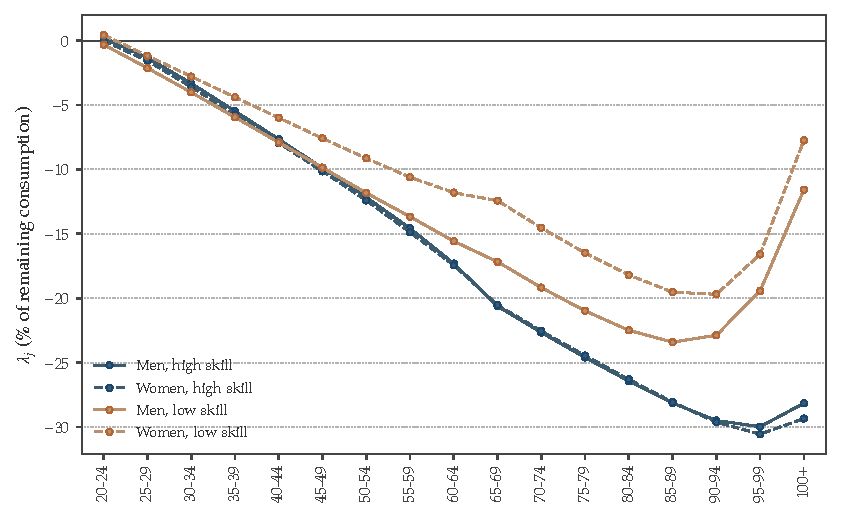
\includegraphics[width=0.85\textwidth]{Figures/cf_lambda_age_cf0.pdf}
\fignote{0.9}{The figure reports age-specific consumption equivalents, $\lambda_j$, comparing same-age residents of CF0 with those of the 2020 baseline. Negative values indicate lower welfare under CF0, expressed as a percentage of remaining lifetime consumption. High-skill individuals are represented by \serone{high skill} and low-skill individuals by \sertwo{low skill}; solid lines represent men and dashed lines women. Comparisons are between stationary equilibria and do not capture transition effects.}
\end{figure}

\paragraph{Welfare differences across demographic groups.}
The age-specific welfare losses under CF0 also differ by sex and education. Beyond age 50, losses are largest for high-education men and women, exceeding $20\%$ of remaining consumption at ages 65--69. At these ages, the losses are approximately $17\%$ for low-education men and $12\%$ for low-education women. This pattern is consistent with differences in the composition of retirement resources. High-education households accumulate more assets and are therefore more exposed to the lower equilibrium return on savings. In contrast, low-education women hold fewer assets and rely more heavily on pension benefits, which increase by nearly $20\%$ under CF0. The flat pension thus provides greater protection against the decline in returns to savings for households that depend more heavily on pension income.

The small newborn welfare differences under CF0 vary across demographic groups. Low-education women experience the largest gain ($0.43\%$), while low-education men experience the largest loss ($0.31\%$). These differences may reflect two features of the model. First, the increase in flat pension benefits is relatively more valuable to households with lower lifetime earnings. Second, differences in survival across sex and education affect the expected duration of pension receipt. In the baseline mortality inputs, the education gradient in survival emerges in the mid-fifties for men, whereas for women it appears only from age 70, partly because of the upper bound imposed on baseline survival probabilities, as discussed in Section~\ref{subsec:validation}. These mechanisms may contribute to the differences in newborn welfare, but their individual contributions have not been quantified. Given the small magnitude of the welfare changes and the sensitivity of the survival probabilities to their construction, the ranking across demographic groups should be interpreted cautiously.

\subsection{Benefit Reduction}
\label{subsec:exp_kappa_taum}

Under CF1, we reduce the pension replacement rate from $\kappa=0.40$ to $\kappa=0.1846$, a reduction of approximately $54\%$, to restore the contribution rate to its 2020 level. From the PAYG financing condition~\eqref{eq:pension_contribution}, the required replacement rate is given by $\kappa=\tau^p_{2020}/(N^R/N^W)$. Using the CF0 dependency ratio of $0.3064$ yields a replacement rate of approximately $0.1846$. The resulting equilibrium contribution rate is $5.660\%$, compared with the baseline value of $5.658\%$. The small difference reflects changes in the dependency ratio arising from endogenous survival.

\paragraph{Aggregate and welfare effects.}
Relative to CF0, reducing the replacement rate lowers pension benefits per retiree by approximately $47\%$, from $0.569$ to $0.303$. As households rely more heavily on private savings to finance retirement, aggregate capital increases from $10.04$ to $12.82$. The resulting capital deepening raises the wage by $7\%$ and reduces the annual interest rate from $6.82\%$ to $5.89\%$. Newborn welfare increases by $8.29\%$ of lifetime consumption relative to CF0, with gains ranging from $7.82\%$ to $9.30\%$ across demographic groups. Relative to the 2020 baseline, the aggregate newborn welfare gain is $8.41\%$.

The welfare gains are consistent with the return differential emphasized by \citet{Aaron1966}. In a stationary PAYG system, the implicit return on contributions is associated with population growth, approximately $1.5\%$ annually in the aged economy, compared with a market interest rate of $5.9\%$. Reducing the size of the pension system allows households to allocate more resources toward private savings, which offer a higher return in the calibrated economy. The resulting capital accumulation also raises wages, reinforcing the welfare gains for newborn households.

Relative to CF0, reducing the replacement rate lowers pension benefits per retiree by approximately $47\%$, from $0.569$ to $0.303$. The reduction in pension benefits encourages households to accumulate more private savings to finance retirement. Aggregate capital increases from $10.04$ to \$12.82, raising the wage by $7\%$ and reducing the annual interest rate from $6.82\%$ to $5.89\%$. The combination of higher wages and lower pension contributions increases after-tax labor income, while the larger capital stock reduces the return on savings. In the resulting equilibrium, newborn welfare increases by $8.29\%$ of lifetime consumption relative to CF0, with gains ranging from $7.82\%$ to $9.30\%$ across demographic groups. Relative to the 2020 baseline, the aggregate newborn welfare gain is $8.41\%$.

\paragraph{Transition effects.}
The $8.29\%$ welfare gain applies to newborns in the reformed stationary equilibrium relative to CF0. It does not account for the welfare consequences of introducing the reform for generations already alive. In particular, individuals who contributed under the previous pension rules could experience substantial losses if their retirement benefits were subsequently reduced. These effects depend on the transition between equilibria, which we do not model. The steady-state welfare gains therefore do not imply that the benefit reduction constitutes a Pareto improvement.

\paragraph{Welfare differences by age.}
Panel~(a) of Figure~\ref{fig:cf_lambda_menu} shows that the welfare effects of the benefit reduction vary substantially with age. Relative to CF0, newborns and young workers experience welfare gains of $7$--$9\%$ of remaining lifetime consumption, while older individuals experience increasingly large losses. At ages 65--69, these losses range from $3.7\%$ for high-education men to $21\%$ for low-education women. The age at which the welfare effect becomes negative also differs across groups. Low-education women experience losses beginning at ages 45--49, followed by low-education men at ages 50--54, high-education women at ages 55--59, and high-education men at ages 60--64. These differences are consistent with the relative importance of pension benefits and private savings across demographic groups. Individuals who rely more heavily on pension income are more adversely affected by the benefit reduction, while those with greater private savings benefit more from the changes in equilibrium factor prices.

\begin{figure}[H]
\centering
\caption{Age-Specific Welfare Effects of Benefit Reduction and Later Retirement}
\label{fig:cf_lambda_menu}
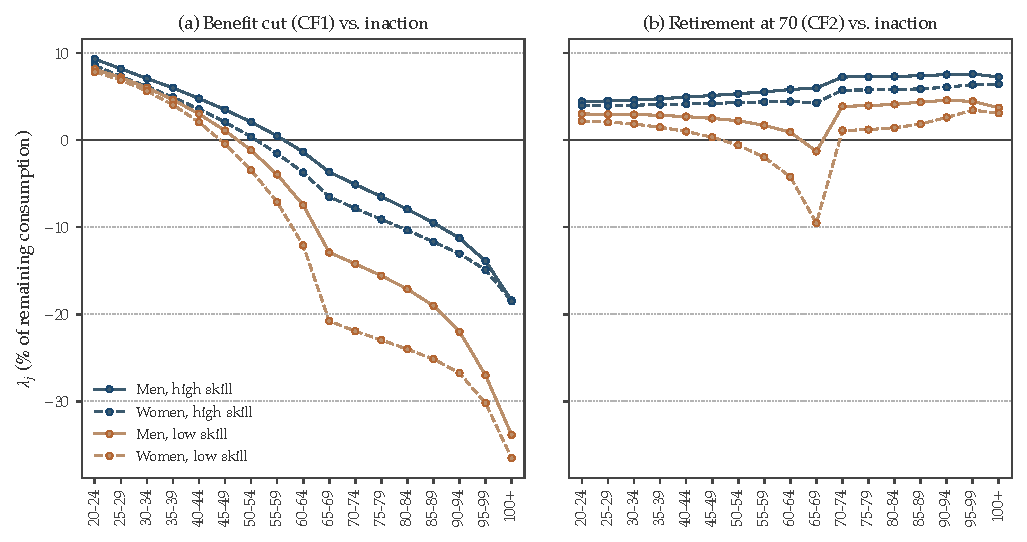
\includegraphics[width=\textwidth]{Figures/cf_lambda_age_menu.pdf}
\fignote{0.94}{The figure reports age-specific consumption equivalents, $\lambda_j$, comparing same-age residents of each reform economy with those under the contribution-rate adjustment (CF0). Panel (a) shows the benefit reduction (CF1), which lowers the replacement rate from $0.40$ to $0.1846$. Panel (b) shows the retirement-age increase (CF2), from 65 to 70. Positive values indicate higher welfare under the reform relative to CF0, expressed as a percentage of remaining lifetime consumption. High-skill individuals are represented by \serone{high skill} and low-skill individuals by \sertwo{low skill}; solid lines represent men and dashed lines women. These comparisons are between stationary equilibria and exclude transition effects. The productivity profiles for ages 65--69 in CF2 are estimated from individuals employed at those ages and may not represent the productivity of individuals affected by the reform.}
\end{figure}


\subsection{Retirement-Age Increase}
\label{subsec:cf_retirement}

Under CF2, we increase the retirement age from 65 to 70, extending the working-age period and delaying pension eligibility by five years. The replacement rate remains at $\kappa=0.40$. Relative to CF0, the ratio of retirees to working-age individuals falls from $0.3064$ to $0.2195$, reducing the pension contribution rate from $12.26\%$ to $8.78\%$. Pension benefits per retiree increase slightly, from $0.569$ to $0.580$, reflecting an increase in average labor income per working-age individual.


\paragraph{Aggregate effects.}
Relative to CF0, raising the retirement age increases aggregate effective labor by approximately $9\%$, from $9.44$ to $10.31$. Aggregate capital increases by a similar proportion, from $10.04$ to $10.96$, leaving the capital--labor ratio virtually unchanged. Consequently, the equilibrium wage and interest rate remain nearly identical to those under CF0. Aggregate output increases from $15.48$ to $16.91$, an increase of approximately $9\%$. Thus, unlike the benefit reduction, which generates substantial capital deepening and changes in factor prices, the retirement-age increase primarily expands aggregate production while reducing the pension contribution rate.

\paragraph{Newborn welfare.}
Raising the retirement age to 70 increases aggregate newborn welfare by $3.11\%$ of lifetime consumption relative to the contribution-rate adjustment (CF0), with gains ranging from $2.19\%$ for low-education women to $4.43\%$ for high-education men (Table~\ref{tab:cf_welfare}). However, newborn welfare under CF2 is $5.45\%$ lower than under the benefit reduction (CF1). The ranking $\mathrm{CF1}\succ\mathrm{CF2}\succ\mathrm{CF0}$ holds for all four demographic types. Unlike CF1, the retirement-age increase does not generate substantial additional capital deepening relative to CF0, leaving equilibrium factor prices nearly unchanged. Instead, it reduces pension contributions while delaying pension eligibility and extending the ages at which individuals can work. The resulting welfare gains are positive but smaller than those obtained through benefit reduction.


\paragraph{Welfare differences by age.}
Panel~(b) of Figure~\ref{fig:cf_lambda_menu} shows that the welfare effects of raising the retirement age differ substantially across age and education groups. Relative to CF0, low-education women experience welfare losses beginning at ages 50--54, reaching $9.5\%$ of remaining lifetime consumption at ages 65--69. Low-education men experience a smaller loss of $1.3\%$ at ages 65--69. In contrast, high-education individuals experience welfare gains at all ages, ranging from $3.9\%$ to $7.6\%$. Individuals aged 70 and older also benefit from the reform, which slightly increases pension benefits without changing their retirement status. These differences are consistent with the substantial variation in labor productivity at older ages. At ages 65--69, estimated productivity is $1.80$ and $1.39$ efficiency units for high-education men and women, respectively, compared with $0.88$ and $0.64$ for their low-education counterparts. The lower potential earnings of low-education workers make the delay in pension eligibility and the extension of working age more costly for these groups.

\subsection{Decomposition of Welfare Effects}
\label{subsec:cf_decomposition}

We decompose the change in newborn expected lifetime utility in each counterfactual relative to the 2020 baseline into three components. First, we solve the household problem under the experiment's direct changes, holding factor prices $(r,w)$, the pension contribution rate $\tau^p$, and pension benefits $\overline{pen}$ at their baseline values. Second, we introduce the experiment's equilibrium factor prices while keeping the fiscal variables unchanged. Third, we also introduce the experiment's equilibrium contribution rate and pension benefits. The changes in lifetime utility between successive steps measure the direct household, factor-price, and fiscal components, respectively. These intermediate calculations do not impose market clearing. The three components sum to the total welfare change, but their individual contributions depend on the order in which the changes are introduced. We report the decomposition in units of expected lifetime utility rather than consumption equivalents, which are not additive across the three components.

\begin{table}[H]
\centering
\caption{Decomposition of changes in newborn welfare}
\label{tab:cf_decomposition}
\begin{tabular}{@{}lcccc@{}}
\toprule
 & \thead{Direct effect} & \thead{Factor prices} & \thead{Fiscal variables} & \thead{Total} \\
\midrule
CF0: Contribution-rate adjustment & $0$ & $+3.247$ & $-3.180$ & $+0.067$ \\
CF1: Benefit reduction            & $0$ & $+5.017$ & $-1.035$ & $+3.983$ \\
CF2: Retirement-age increase      & $-0.432$ & $+3.310$ & $-1.348$ & $+1.530$ \\
\bottomrule
\end{tabular}
\vspace{0.5em}
\begin{minipage}{0.92\textwidth}
\footnotesize
\textit{Notes.} Entries report changes in birth-share-weighted expected lifetime utility relative to the 2020 baseline, whose level is $340.60$. The direct effect measures the change from the experiment's policy parameters holding factor prices and fiscal variables at their baseline values. The factor-price component introduces the experiment's equilibrium interest rate and wage, while maintaining baseline fiscal variables. The fiscal component introduces the experiment's equilibrium pension contribution rate and benefits. The components sum to the total change, up to rounding. Intermediate calculations do not impose market clearing, and the decomposition depends on the order in which equilibrium changes are introduced. Values are expressed in lifetime utility units, not consumption equivalents.
\end{minipage}
\end{table}

The first two rows of Table~\ref{tab:cf_decomposition} show that changes in factor prices increase newborn welfare under both CF0 and CF1, but these gains are partially offset by changes in pension contributions and benefits. The direct component is zero in both experiments because neither population growth nor the replacement rate enters the household optimization problem when factor prices and fiscal variables are held fixed. Under CF0, the positive factor-price contribution of $3.247$ is almost entirely offset by the negative fiscal contribution of $3.180$, leaving a small net welfare gain of $0.067$ utility units. Under CF1, the factor-price contribution is larger ($5.017$), consistent with the greater capital deepening induced by the benefit reduction. The negative fiscal contribution is also smaller ($-1.035$), resulting in a net welfare gain of $3.983$ utility units.

The third row of Table~\ref{tab:cf_decomposition} shows that the retirement-age increase (CF2) has a negative direct welfare effect of $0.432$ utility units. Unlike CF0 and CF1, this reform changes the household optimization problem directly by delaying pension eligibility and extending the ages at which individuals can supply labor. Holding factor prices and fiscal variables at their 2020 baseline values, these changes reduce newborn welfare. The factor-price component contributes $3.310$ utility units, while the fiscal component reduces welfare by $1.348$ units. Together, these effects yield a net welfare gain of $1.530$ utility units relative to the 2020 baseline. Thus, the positive overall welfare effect arises from the combination of direct household responses and changes in equilibrium prices and pension finances, rather than from the direct adjustment to retirement age alone.


\subsection{Caveats}
\label{subsec:exp_caveats}

The experiments compare stationary equilibria and do not capture transition paths or the welfare effects on generations alive when a reform is introduced. Demographic aging is implemented by changing the population growth rate $n_p$ to reproduce the projected 2050 dependency ratio, while holding baseline survival probabilities and the composition of entering cohorts fixed. Thus, the experiments do not incorporate projected changes in mortality or educational composition. In addition, the baseline survival probabilities truncate the education gradient for women aged 50--69, as discussed in Section~\ref{subsec:validation}.

The quantitative results are also conditional on the model's fiscal structure and numerical implementation. We do not consider financing pensions through general tax revenues or government debt, which would require modifying the PAYG financing rule. Government debt instead adjusts to balance the general government budget, yielding debt ratios of $107$--$124\%$ of annual output, compared with approximately $50\%$ in Mexico. All equilibria are computed on the same numerical grid, so the reported levels are subject to numerical approximation. Finally, we do not evaluate health-policy reforms. Health capital remains close to its upper bound in the calibrated model, limiting the scope for additional health accumulation under the current specification, as discussed in Section~\ref{subsec:health_block_evidence}.


% ======================================================================


%% ====================================================================
%% SECTION 8 — CONCLUSION
%% ====================================================================

\section{Conclusion}
\label{sec:conclusion}

This paper examines the macroeconomic and welfare consequences of demographic aging and alternative pension adjustments in Mexico using a calibrated stochastic overlapping-generations model with endogenous health and heterogeneity by sex and education. We find that demographic aging under contribution-rate adjustment (CF0) leaves aggregate newborn welfare nearly unchanged relative to the 2020 baseline. However, comparisons between stationary equilibria reveal increasingly large welfare losses among older residents. Benefit reduction (CF1) and retirement-age increase (CF2) both improve newborn welfare relative to CF0, although their distributional consequences differ across ages and demographic groups.

Under the contribution-rate adjustment (CF0), demographic aging raises the pension contribution rate from $5.66\%$ to $12.26\%$. At the same time, capital deepening increases wages and lowers the interest rate. Together with the changes in pension contributions and benefits, these general-equilibrium adjustments leave aggregate newborn welfare nearly unchanged, with a gain of $0.14\%$ relative to the 2020 baseline. However, the welfare comparisons become increasingly negative at older ages, consistent with the greater exposure of asset-holding households to the lower return on savings.

The two pension reforms generate larger newborn welfare gains than the contribution-rate adjustment (CF0). Reducing the replacement rate from $0.40$ to approximately $0.185$ (CF1) restores the contribution rate to its 2020 level and increases aggregate newborn welfare by $8.29\%$ relative to CF0. Raising the retirement age from 65 to 70 (CF2) reduces the contribution rate to $8.78\%$ and generates a newborn welfare gain of $3.11\%$. All four sex-education groups rank CF1 above CF2 and CF2 above CF0. However, the age-specific welfare comparisons differ. Benefit reduction generates losses among older residents who depend more heavily on pension income, while the retirement-age increase generates losses among low-education individuals approaching retirement, particularly women. Thus, the reform that produces the largest newborn welfare gains does not necessarily improve welfare for residents at other ages.

Our findings are subject to several limitations. First, we compare stationary equilibria rather than transition paths, so the welfare gains for newborns do not account for the consequences of introducing pension reforms for generations already alive. Second, the model assumes a closed economy, in which changes in domestic capital accumulation affect equilibrium wages and interest rates. International capital mobility could alter these adjustments and their welfare implications. Finally, the model abstracts from informal employment, which may affect both pension financing and the distributional consequences of reform.



%% ====================================================================
%% BIBLIOGRAPHY
%% ====================================================================
\bibliography{references}

%% ====================================================================
%% APPENDICES
%% ====================================================================
\begin{appendices}

\section{Model Appendix: Derivations and Optimality Conditions}
\label{app:model}

This appendix collects two derivations behind the model of Section~\ref{sec:model}: the comparison of multiplicative and additive health amenities that motivates the specification of preferences, and the optimality conditions of the household problem.

\subsection{The Amenity: Multiplicative versus Additive}
\label{app:amenity}

Section~\ref{subsec:preferences} states that the multiplicative amenity creates an income gradient in the willingness to pay for health that an additive amenity lacks by construction. This appendix records the derivations behind that claim.

Scaling the GHH aggregator by $\Omega(h)$ makes the marginal utility of consumption depend on health,
\begin{equation}
\label{eq:u_ch}
u_{ch} \;=\; \Omega'(h)\,\bigl(c-v(\ell)\bigr)^{-\gamma} \;\geq\; 0,
\end{equation}
with strict inequality whenever $\Xi > 0$. The sign holds at every state, since $\Omega' \geq 0$ and $(c - v(\ell))^{-\gamma} > 0$ irrespective of the bracket in~\eqref{eq:utility}. Health is a state rather than a within-period choice, so this complementarity reaches the medical-spending decision indirectly: through $u_h$ in the health envelope condition~\eqref{eq:env_h}, which supplies the marginal continuation value in~\eqref{eq:foc_m}, and through the dependence of next period's $u_c$ on $h'$ in the consumption Euler equation~\eqref{eq:euler}.

Had the amenity entered the composite additively, as $u = \bigl[(c + s(h) - v(\ell))^{1-\gamma} - 1\bigr]/(1-\gamma)$ with $s' > 0$, the same cross-partial would carry the opposite sign,
\[
u_{ch} \;=\; -\gamma\, s'(h)\, \bigl(c + s(h) - v(\ell)\bigr)^{-\gamma-1} \;<\; 0 .
\]
The sign of $u_{ch}$ is not, however, the object that governs behavior. Medical spending responds to the marginal rate of substitution between health and consumption, which is what enters the medical-spending condition~\eqref{eq:foc_m}. Under the additive form that ratio is
\[
\frac{u_h}{u_c} \;=\; \frac{s'(h)\,\bigl(c+s(h)-v(\ell)\bigr)^{-\gamma}}{\bigl(c+s(h)-v(\ell)\bigr)^{-\gamma}} \;=\; s'(h),
\]
independent of consumption. Health and consumption are perfect substitutes inside the composite, so the willingness to pay for health carries no income gradient; the negative $u_{ch}$ above is the concavity of the outer aggregator and by itself moves nothing. Under the multiplicative form the same ratio is
\[
\frac{u_h}{u_c} \;=\; \frac{\Omega'(h)}{\Omega(h)}\left[\frac{z^{1-\gamma}-1}{1-\gamma} + \chi\right] z^{\gamma}, \qquad z \equiv c - v(\ell),
\]
which is increasing in $c$ whenever $1 + \gamma\bigl[(z^{1-\gamma}-1)/(1-\gamma) + \chi\bigr]z^{\gamma-1} > 0$. The condition holds at every state at which the bracket in~\eqref{eq:utility} is nonnegative, and can fail only inside the region where that bracket is negative, that is, at states the household ranks below not being alive.

The two forms also differ at the boundary of the feasible set. Because the amenity multiplies the aggregator, $u_c = \Omega(h)\,(c-v(\ell))^{-\gamma} \to \infty$ as $c \downarrow v(\ell)$, so consumption satisfies an Inada condition. Under an additive amenity the singularity sits instead at $c = v(\ell) - s(h)$, which is strictly negative whenever $s(h) > v(\ell)$. The Inada point is then unreachable, $u_c$ stays finite as $c \to 0$, and a household can be close to indifferent between consuming and not.

\subsection{Household Optimality Conditions}
\label{app:focs}

This appendix states the first-order, envelope, and Kuhn--Tucker conditions of the worker's problem~\eqref{eq:worker_bellman} and the retiree's problem~\eqref{eq:retiree_bellman}. Let $q_j$ denote the multiplier on the budget constraint, and recall that the two nodes $h'_k$ of the health lottery~\eqref{eq:health_lom_shock} are functions of $(m, h)$ through $\tilde h$. At an optimum at which the $\min$ and $\max$ operators in~\eqref{eq:health_lom_shock} are slack at both nodes, $\partial h'_k / \partial m = \partial H_j / \partial m$ and $\partial h'_k / \partial h = \partial \tilde h / \partial h$ for both $k$, with the derivatives given in~\eqref{eq:dh_dh}. The interior first-order conditions are
\begin{align}
\text{Consumption:} \quad & u_c(c, \ell, h) \;=\; q_j (1 + \tau^c), \label{eq:foc_c}\\
\text{Labor:} \quad & -u_\ell(c, \ell, h) \;=\; q_j\, w\, \nu_j(h, \eta;\, g, \theta)\,(1-\tau^\omega-\tau^p), \label{eq:foc_l}\\
\text{Savings:} \quad & q_j \;=\; \beta \sum_{k \in \{0,1\}} \Pr(k \mid j)\; \psi_{j+1}^{g,\theta}(h'_k)\, \E\bigl[V_{a, j+1}(a', h'_k, \eta';\, g, \theta) \mid \eta\bigr], \label{eq:foc_a}\\
\text{Medical spending:} \quad & q_j (1 + \tau^m)
\;=\; \beta\, \frac{\partial H_j(m,h)}{\partial m} \sum_{k \in \{0,1\}} \Pr(k \mid j)\Bigl\{
\bigl(\psi_{j+1}^{g,\theta}\bigr)'(h'_k)\, \E[V_{j+1}(a', h'_k, \eta';\, g, \theta) \mid \eta] \notag\\
&\qquad\qquad\qquad\qquad +\, \psi_{j+1}^{g,\theta}(h'_k)\, \E[V_{h, j+1}(a', h'_k, \eta';\, g, \theta) \mid \eta]
\Bigr\}. \label{eq:foc_m}
\end{align}
Condition~\eqref{eq:foc_m} states the two returns to medical spending that the model keeps distinct---a survival return, through $(\psi^{g,\theta}_{j+1})'$ multiplying the level of the continuation value, and a health-capital return, through $\psi^{g,\theta}_{j+1}$ multiplying its marginal value in health---each averaged over the two nodes of the health lottery. Because $\varsigma$ shifts the struck node down by a constant, the marginal product of spending is common to the two nodes and factors out; what differs across nodes is the point at which the survival schedule and the continuation value are evaluated. If the floor $\underline h$ binds at the struck node, that node's health no longer responds to $m$ and the $k=1$ term drops from the right-hand side of~\eqref{eq:foc_m}.

\paragraph{Envelope conditions.} For the worker's problem ($j < j_R$),
\begin{align}
V_{a, j}(a, h, \eta;\, g, \theta) &\;=\; q_j \cdot \bigl(1 + r(1-\tau^k)\bigr), \label{eq:env_a}\\
V_{h, j}(a, h, \eta;\, g, \theta) &\;=\; u_h(c, \ell, h) + q_j\, w\, \nu_j(h, \eta;\, g, \theta)\, \varrho\, \ell\, (1-\tau^\omega-\tau^p) \notag\\
&\qquad +\, \beta\, \frac{\partial \tilde h}{\partial h} \sum_{k \in \{0,1\}} \Pr(k \mid j)\Bigl\{ \bigl(\psi_{j+1}^{g,\theta}\bigr)'(h'_k)\, \E[V_{j+1}(a', h'_k, \eta';\, g, \theta) \mid \eta] \notag\\
&\qquad\qquad\qquad\qquad\qquad +\, \psi_{j+1}^{g,\theta}(h'_k)\, \E[V_{h, j+1}(a', h'_k, \eta';\, g, \theta) \mid \eta] \Bigr\}, \label{eq:env_h}
\end{align}
with $\partial \tilde h / \partial h$ from~\eqref{eq:dh_dh}. The second term is the wage return to health. Its slope $\varrho$ is common to the two skill groups, so any cross-group difference in the earnings value of health operates through the wage bill $w\,\nu_j\,\ell$---through the intercept $\theta$ and the profile $e^{g,\theta}_j$---rather than through a differential return: health is worth more, in earnings, to workers whose time is worth more. For the retiree's problem ($j \geq j_R$), $\ell = 0$ and that term vanishes:
\begin{align}
V_{a, j}^{R}(a, h, \eta;\, g, \theta) &\;=\; q_j \cdot \bigl(1 + r(1-\tau^k)\bigr), \label{eq:env_a_ret}\\
V_{h, j}^{R}(a, h, \eta;\, g, \theta) &\;=\; u_h(c, 0, h) \notag\\
&\qquad +\, \beta\, \frac{\partial \tilde h}{\partial h} \sum_{k \in \{0,1\}} \Pr(k \mid j)\Bigl\{ \bigl(\psi_{j+1}^{g,\theta}\bigr)'(h'_k)\, \E[V_{j+1}(a', h'_k, \eta';\, g, \theta) \mid \eta] \notag\\
&\qquad\qquad\qquad\qquad\qquad +\, \psi_{j+1}^{g,\theta}(h'_k)\, \E[V_{h, j+1}(a', h'_k, \eta';\, g, \theta) \mid \eta] \Bigr\}. \label{eq:env_h_ret}
\end{align}
At the terminal age $j = J$, $\psi^{g,\theta}_{J+1} \equiv 0$ kills the continuation terms; the envelopes remain well defined since $a_J' = m_J = 0$.

\paragraph{Euler equation.} Combining~\eqref{eq:foc_a} with~\eqref{eq:env_a} one period ahead and~\eqref{eq:foc_c},
\begin{equation}
\label{eq:euler}
u_c(c, \ell, h) \;=\; \beta\, \bigl(1 + r(1-\tau^k)\bigr) \sum_{k \in \{0,1\}} \Pr(k \mid j)\; \psi_{j+1}^{g,\theta}(h'_k)\, \E\bigl[u_c(c'_k, \ell'_k, h'_k) \mid \eta\bigr],
\end{equation}
where $(c'_k, \ell'_k)$ are next-period policies evaluated at the node-$k$ health state.

\paragraph{Consumption--leisure condition.} Combining~\eqref{eq:foc_c} and~\eqref{eq:foc_l},
\begin{equation}
\label{eq:cons_leisure}
\frac{-u_\ell(c, \ell, h)}{u_c(c, \ell, h)}
\;=\;
\frac{w\, \nu_j(h, \eta; g, \theta)(1-\tau^\omega-\tau^p)}{1 + \tau^c},
\end{equation}
where the amenity cancels from the left-hand side, since $\Omega(h)$ scales $u$ uniformly: $-u_\ell/u_c = v'(\ell)$.

\paragraph{Kuhn--Tucker for the borrowing constraint.}
The constraint $a' \geq 0$ generates a non-negative multiplier and turns the savings condition~\eqref{eq:foc_a} into the weak inequality
\begin{equation}
\label{eq:kt_borrowing}
q_j \;\geq\; \beta \sum_{k \in \{0,1\}} \Pr(k \mid j)\; \psi_{j+1}^{g,\theta}(h'_k)\, \E\bigl[V_{a, j+1}(a', h'_k, \eta';\, g, \theta) \mid \eta\bigr], \qquad a' \geq 0,
\end{equation}
with complementary slackness: the product of the gap and $a'$ is zero.

\paragraph{Kuhn--Tucker for medical spending.}
The constraint $m \geq 0$ turns~\eqref{eq:foc_m} into the weak inequality
\begin{equation}
\label{eq:kt_medical}
q_j (1 + \tau^m)
\;\geq\;
\beta\, \frac{\partial H_j(m,h)}{\partial m} \sum_{k \in \{0,1\}} \Pr(k \mid j)\Bigl\{
\bigl(\psi_{j+1}^{g,\theta}\bigr)'(h'_k)\, \E[V_{j+1}(\cdot) \mid \eta]
+ \psi_{j+1}^{g,\theta}(h'_k)\, \E[V_{h, j+1}(\cdot) \mid \eta]
\Bigr\},
\end{equation}
for $m \geq 0$, with complementary slackness. The cap $h'_k \leq \bar h$ in~\eqref{eq:health_lom_shock} is slack wherever $\overline{H}_j m^{\zeta_h} < \bar h$, by the asymptote property of~\eqref{eq:health_production_deficit}; where it binds it introduces a non-negative multiplier $\mu_{\bar h} \geq 0$ with complementary slackness
\begin{equation}
\label{eq:kt_healthcap}
\mu_{\bar h}\,(\bar h - h'_0) \;=\; 0, \qquad h'_0 \leq \bar h, \qquad \mu_{\bar h} \geq 0,
\end{equation}
entering the medical-spending condition as a subtracted term $\mu_{\bar h}\, \partial H_j/\partial m$ on the right-hand side of~\eqref{eq:kt_medical}. At an interior optimum with $m > 0$ and both nodes strictly inside $(\underline h, \bar h)$, all inequalities hold with equality and~\eqref{eq:foc_m} is recovered.

\section{Estimation Details}
\label{app:estimation}

This appendix supports the estimator of Section~\ref{subsec:secondstep_smm}. It states the objective and the weighting choice, describes the algorithm that computes the equilibrium and the state space every reported number is computed on, and gives the reasons no standard errors are reported.

\paragraph{The estimator is deterministic.} The state space is discretized and the stationary distribution over $(j,g,\theta,a,h,\eta)$ is computed by forward iteration, so every model moment is an exact distribution-weighted functional rather than a Monte Carlo average over simulated panels. The objective is therefore deterministic---re-evaluating it at the same parameter vector returns the same value---the asymptotic theory is that of classical minimum distance with no simulation-inflation term, and any non-smoothness the optimizer meets is a property of the model rather than of sampling noise. What remains is discretization: moments are kinked wherever mass crosses a grid cell.

\paragraph{Computing the equilibrium.} The equilibrium of Definition~\ref{def:equilibrium} is the fixed point of three nested maps. The inner map is the household problem, solved by backward induction on the finite-horizon Bellman equations~\eqref{eq:worker_bellman} and~\eqref{eq:retiree_bellman} together with the savings and medical-spending conditions~\eqref{eq:foc_a}--\eqref{eq:foc_m} of Appendix~\ref{app:focs}, with labor supply concentrated out through the intratemporal condition~\eqref{eq:cons_leisure} and constrained maximization over the remaining controls $(a', m)$. The middle map iterates the population measure~\eqref{eq:lom} jointly with the cohort weights~\eqref{eq:cohort_weights} and the health-dependent survival schedule~\eqref{eq:avg_survival} to their mutual fixed point, which is condition 10 of the definition. The outer map adjusts the capital--labor ratio until the factor-price conditions~\eqref{eq:foc_r}--\eqref{eq:foc_w} and the capital-market condition~\eqref{eq:capital_market} clear, with the contribution rate and the stationary debt level moving through~\eqref{eq:pension_contribution} and~\eqref{eq:gov_stationary}. That outer map is not nested inside the estimation objective: parameters are obtained at fixed anchor prices, as Section~\ref{subsec:secondstep_smm} describes, and the three maps run jointly only at the estimates and in the experiments.  The endogenous grid method is not available here. Medical spending enters the continuation value non-separably and through its level, since the survival derivative in~\eqref{eq:foc_m} multiplies $\E[V_{j+1}]$ rather than only its marginal value, and next-period health is itself a control. The end-of-period state is therefore not exogenous and the Euler equation cannot be inverted in closed form. At the calibrated baseline the supporting residuals are small: the largest Euler-equation residual across interior cells is $10^{-7.5}$ in marginal-utility units, the goods and capital markets clear to within $8\times10^{-5}$ of output and capital respectively, and the cohort-share invariant implied by~\eqref{eq:avg_survival} holds to $3\times10^{-15}$.

\paragraph{Objective and weighting.} The estimator solves
\begin{equation}
\label{eq:smm_objective}
\widehat\Theta_{\mathrm{MD}} \;=\; \arg\min_{\Theta}\; \sum_{k=1}^{10} \left( \frac{m_k^{\mathrm{mod}}(\Theta) - m_k^{\mathrm{dat}}}{m_k^{\mathrm{dat}}} \right)^{2} \;+\; \mathcal{P}(\Theta),
\end{equation}
that is, minimum distance with $W=\operatorname{diag}\bigl(1/(m^{\mathrm{dat}})^2\bigr)$. The term $\mathcal{P}$ is a smooth penalty, zero over almost all of the admissible set, that excludes the region in which some household would assign negative value to survival; it binds nowhere near the estimates, where no household does. We do not use inverse-variance weighting, $W=\operatorname{diag}(1/\mathrm{SE}^2)$, for two reasons. The standard errors are not commensurable across this target set: one target is a convention with no sampling error at all, and the survey moments mix cluster-robust, delta-method, and bootstrap objects. And inverse-variance weighting turns the estimator into a matcher of $t$-statistics rather than of economic magnitudes---at the starting values it concentrated the objective on a single precisely estimated survey moment, leaving the moments that carry the paper's mechanism nearly weightless. Equal proportional weighting prices a ten-percent miss identically wherever it occurs and carries no efficiency claim. Nine parameters against ten moments over-identifies the system by one, but the over-identifying restriction is the survival-anchor overlap described in Section~\ref{subsec:secondstep_smm} rather than a restriction the theory imposes on the data, so we report no over-identification test. Nor do we claim a numerical rank condition at the estimates: two parameters sit at boundaries of the admissible set, where only one-sided variation exists. Proportional weights on two survival levels near one make the sign of their small difference nearly costless.

\paragraph{Inference.} We report point estimates without standard errors. The numerical derivatives that the minimum-distance sandwich formula requires are not stable here---the derivative of one of the two moments that dominate the objective at the estimates is not sign-stable across candidate step sizes, so a standard error built on it would be spuriously precise---and two estimates sit at boundaries of the admissible set, where the unconstrained sandwich does not apply in any case. The nine parameters are searched under a logit transform onto their admissible intervals, so a bound is an asymptote the search approaches without attaining. The two driven to the bottom of their intervals are the amenity scale, admissible on $[10^{-4},\,5]$, and the shock arrival rate, on $[0.01,\,0.436]$. A step-size study and a treatment of the two boundary estimates are prerequisites to reporting inference rather than robustness checks on it. Until then the fit of Table~\ref{tab:moment_match_md}, rather than a $t$-statistic, is the measure of precision on offer.

\paragraph{Optimizer and state space.} The outer search is a derivative-free simplex method terminated by a no-further-improvement rule rather than by a formal convergence criterion. All reported numbers---estimates, fit, validation, and the experiments of Section~\ref{sec:experiments}---are computed on the coarser of two state-space grids. That grid carries $100$ asset nodes on a geometric mesh reaching $300$, ten health nodes, five nodes for the persistent productivity shock, and twenty for medical spending; the finer grid raises the last three to fifteen, seven and eighty. The productivity process~\eqref{eq:ar1} is discretized by the Rouwenhorst method, which matches the persistence of the underlying AR(1) exactly at this node count. The two grids differ in the levels of some moments, so reported levels carry the caveat while cross-economy comparisons, which the paper's results rest on, do not. A polish on the finer grid awaits the health-block specification decision of Section~\ref{sec:conclusion}.

\section{2050 Demographic Inputs: Derivation and Sources}
\label{app:demog2050}

This appendix documents the single input that distinguishes the aged economy of Section~\ref{sec:experiments} from the baseline: the 2050 old-age dependency ratio, its source, and the population growth rate that reproduces it.

\paragraph{Source.} The demographic target for the 2050 experiments of Section~\ref{sec:experiments} is the old-age dependency ratio $65{+}/(20\text{--}64)$ from CONAPO's official population projections for M\'exico \citep[Proyecciones de la Poblaci\'on de M\'exico y de las Entidades Federativas, 2023 revision;][]{CONAPO2023}: $0.3065$ in 2050, against the 2020 census value of $0.1414$ that disciplines the baseline (Section~\ref{subsec:firststep}). The bracketing projections ($0.1746$ in 2030, $0.5064$ in 2070) locate 2050 on a still-steepening path. The 2050 ratio comes from the same CONAPO release as the life tables used in the first step,  The UN World Population Prospects is the natural robustness alternative and changes only the target number.

\paragraph{Method.} The experiment imposes the 2050 population \emph{structure}, not a demographic forecast path, and it does so through the single parameter the baseline already uses for the same purpose. In the stationary population, cohort weights satisfy~\eqref{eq:cohort_weights}, $\phi_{j+1}/\phi_j = \bar\psi_{j+1}/(1+n_p)$, where $n_p$ is the five-year growth rate (the annual rates quoted here are $(1+n_p)^{1/5}-1$) and $\bar\psi_{j+1}$ is the distribution-weighted average survival from band $j$ to band $j+1$---an equilibrium object, since survival is health-modulated. We hold that schedule fixed at its baseline values and bisect $n_p$ against the CONAPO target, which gives $n^{*}_{2050}=1.483\%$ per year. Because the average survivals are themselves equilibrium objects, the bisection only proposes a growth rate; the confirming general-equilibrium solve is what we report. It realizes a dependency ratio of $0.30643$, within $0.024\%$ of the CONAPO value, and the pay-as-you-go identity evaluated at that ratio reproduces the reported contribution rate exactly.

\paragraph{Two arms not run.} Section~\ref{sec:experiments} explains why survival schedules and the birth composition stay at their 2020 values rather than moving to 2050 projections. Two further points complete that argument. A survival arm would need the CONAPO projection stripped to its exogenous component, since the model's own survival is health-modulated and a projected schedule already embeds behaviour. And an education-composition arm would need an external projection of educational attainment, without which it would conflate aging with skill upgrading.


\section{Composition of Out-of-Pocket Medical Spending}
\label{subsec:health_evidence}

We use ENIGH 2018 and 2024 to examine the composition of out-of-pocket medical spending across household income groups. Because ENIGH captures only between $22\%$ and $34\%$ of the corresponding expenditures recorded in national health accounts, we focus on spending composition rather than aggregate expenditure levels. We classify expenditures as preventive, curative, or ambiguous when their purpose cannot be determined from the survey categories. The classification differs between the two survey waves, so comparisons are made across income groups within each year rather than across years.

In 2024, $53.6\%$ of out-of-pocket medical spending was classified as curative, $2.0\%$ as preventive, and the remaining $44.5\%$ as ambiguous, including over-the-counter medicines and dental and optical care. Even if all ambiguous expenditures were classified as preventive, curative care would still account for the majority of spending. Figure~\ref{fig:mot_composition} presents the composition of medical spending across household income deciles in 2018 and 2024.

\begin{figure}[H]
\centering
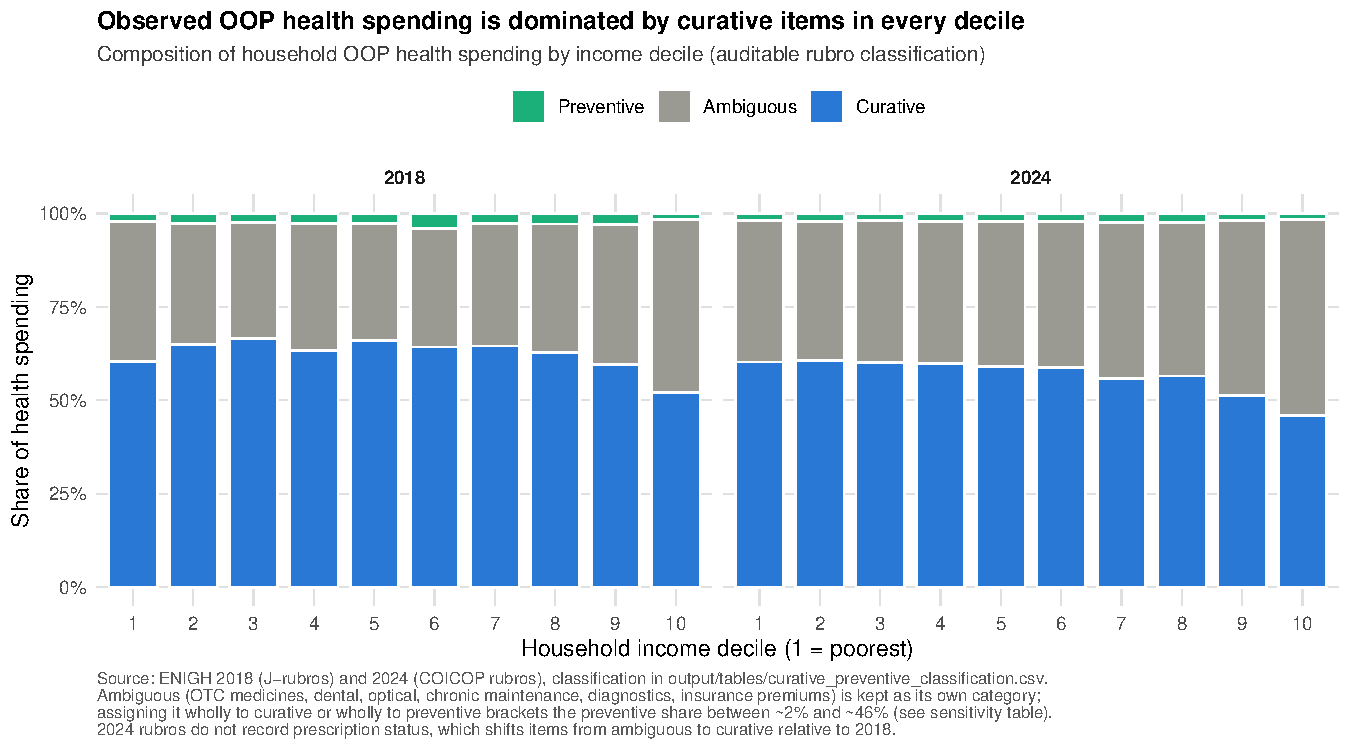
\includegraphics[width=0.95\textwidth]{Figures/fig07_composition.pdf}
\caption{Composition of out-of-pocket medical spending by household income decile, ENIGH 2018 and 2024. Expenditures are classified as preventive, curative, or ambiguous. The ambiguous category includes over-the-counter medicines, dental and optical care, chronic-disease maintenance, diagnostics without a specified purpose, and insurance premiums. In 2024, curative care accounts for the majority of spending even if all ambiguous expenditures are classified as preventive. The classification uses ENIGH J-rubros in 2018 and COICOP categories in 2024, which differ in detail and do not permit direct comparisons of spending composition across years. Comparisons across income deciles within each wave remain valid. Source: ENIGH 2018 and 2024 (INEGI); authors' calculations.}
\label{fig:mot_composition}
\end{figure}

\end{appendices}




\end{document}
